\documentclass[11pt,twoside,a4paper,fleqn]{book} 
%\documentclass[11pt,twoside,a4paper,fleqn,draft]{book} 


%--- Packages to use
%
\usepackage[]{fancyhdr}   
\usepackage[]{natbib}
\usepackage{alltt}
\usepackage{times}
\usepackage{lscape}         % landscape mode of a single page
\usepackage[]{longtable}    % allow tables longer than one page
\usepackage{makeidx}        % index of terms
\usepackage{tabularx}       % allows line breaking in table columns
\usepackage{algorithm}      % for describing algorithms with pseudo-code
\usepackage{algorithmic}
\usepackage{ifthen}
\usepackage{ifpdf}
\usepackage{xr-hyper}
\usepackage{fancyvrb}


%--- Margins
%
\voffset-2.0cm
\headheight16pt
\headsep1.1cm
\textheight22cm
\hoffset-1.3cm
\oddsidemargin2.2cm
\textwidth14.0cm


%--- Headings
%
\pagestyle{fancy}
\renewcommand{\chaptermark}[1]{\markboth{#1}{}}
\renewcommand{\sectionmark}[1]{\markright{\thesection\ #1}}
\fancyhf{}
\fancyhead[LE,RO]{\small{\sc\thepage}}
\fancyhead[LO]{\small{\scshape\rightmark}}
\fancyhead[RE]{\small{\scshape\leftmark}}
\renewcommand{\headrulewidth}{0.5pt}
\renewcommand{\footrulewidth}{0pt}
\fancypagestyle{plain}{%
  \fancyhead{}
  \renewcommand{\headrulewidth}{0pt}
}  


%--- Some layout commands
%
\sloppy
\raggedbottom
\hbadness=10000
\makeindex
\bibliographystyle{agu}


%--- Some fixes

%- To avoid hyperref error:
\newcommand{\theHalgorithm}{\theHchapter.\arabic{algorithm}}

%- Width of the caption in longtable:
\setlength{\LTcapwidth}{0.9\textwidth} 

%- Change brace type for comments in algorithmic
\renewcommand{\algorithmiccomment}[1]{(#1)}


%--- Symbol definitions
%
% This file defines the general math macros.
% Mathematical symbols used only once, or for a particular purpose, 
% should not be included here. Note that the scalar quantities exist 
% in a subscript version, and it is not necessary to define macros for
% all possible subscripts of a variable.
% A lot of macros have been defined for the Rodgers formalism is it
% used extensively.

% If you add new definitions, please try to follow the rules below to
% get a naming scheme as consistent as possible. Just check how a 
% similar macro is defined and use it as an example.

% Patrick Eriksson 2001-03-13

%-----------------------------------------------------------------------------

% Most of the macros are named by putting 3-letters acronyms together. 
% The acronyms are mainly formed by taking the first letter and the two 
% first following consonants. The list below shows the used acronyms.
% Please, if you introduce a new acronym, add it to this list.
%
% altitude     Alt
% angel        Ang
% average      Avr
% azimuthal    Azm
% constant     Cns
% contribution Cnt
% covariance   Cvr
% derivative   Drv
% error        Err
% frequency    Frq
% forward      Frw
% function     Fnc
% identity     Idn
% inverse      Inv
% kernel       Krn
% latitude     Lat       (exception from general naming scheme)
% length       Lng
% longitude    Lon       (exception from general naming scheme)
% matrix       Mtr
% measurement  Msr
% model        Mdl
% partial      Prt
% population   Ppl
% pressure     Prs
% radius       Rds
% retrieval/ed Rtr
% sensor       Sns
% size         Sze
% space        Spc
% state        Stt
% style        Stl
% symbol       Smb
% temperature  Tmp
% transfer     Trf
% transpose    Trp
% wavelength   Wvl
% vector       Vct
% zenith       Znt
%
% a priori                              Apr
% monochromatic pencil beam intensity   Mpi
% optical thickness                     Oth
% weighting function                    Wfn

% For other terms or features, use as far as possible complete strings to get 
% macros with clear names.


%--- General math ------------------------------------------------------------

% Vector style
\newcommand{\VctStl}[1]     {\ensuremath{\mathbf{#1}}}

% Matrix style
\newcommand{\MtrStl}[1]     {\ensuremath{\mathbf{#1}}}

% The identity matrix
\newcommand{\IdnMtr}        {\MtrStl{1}}  

% Scalar or matrix inverse
\newcommand{\Inv}           {^{-1}}  

% Vector or matrix transpose
\newcommand{\Trp}           {^T}  

% Size symbol
\newcommand{\SzeSmb}        {\ensuremath{\in}}  

% Vector space
\newcommand{\VctSpc}[1]     {\ensuremath{\mathbf{R}^#1}}

% Matrix space
\newcommand{\MtrSpc}[2]     {\ensuremath{\mathbf{R}^{#1 \times #2}}}

% Vector length (simple)
\newcommand{\VctLng}        {\ensuremath{n}}  
\newcommand{\aVctLng}[1]    {\ensuremath{n_{#1}}}  

% Index (to vector, matrix ...)
\newcommand{\Ind}           {\ensuremath{i}}  
\newcommand{\aInd}[1]       {\ensuremath{i_{#1}}}  

% Differential d
\newcommand{\DiffD}         {\ensuremath{\mathrm{d}}}  

% Partial d
\newcommand{\PartD}         {\ensuremath{\partial}}  

% Real and Imaginary part
\renewcommand{\Re}            {\ensuremath{\mathrm{Re}}}
\renewcommand{\Im}            {\ensuremath{\mathrm{Im}}}

% Ensemble average
\newcommand{\EnsAvr}[1]        {\ensuremath{\left\langle #1 \right\rangle}}

% Absolute Value
\newcommand{\Abs}[1]          {\ensuremath{\left| #1 \right| }}   

% *10^#1
\newcommand{\topowerten}[1]   {\ensuremath{\cdot10^{#1}}}

% degrees
\newcommand{\degree}          {\ensuremath{^\circ}}

% 1/2
\newcommand{\half} {\ensuremath{\textstyle\frac{1}{2}}}


%--- Physical constants ------------------------------------------------------

% Speed of light in vaccum [m/s]
\newcommand{\speedoflight}   {\ensuremath{c}}  

% Planck constant [Js]
\newcommand{\planckCns}      {\ensuremath{h}}  

% Boltzmann constant [J/K]
\newcommand{\boltzmannCns}   {\ensuremath{k_b}}  

% Avogadro's number [molec/kg]
\newcommand{\avogadrosCns}   {\ensuremath{N_a}}  


%--- The Rodgers formalism ---------------------------------------------------

% True (natural) forward model
\newcommand{\trueFrwMdl}       {\ensuremath{F}}  

% Discrete forward model
\newcommand{\FrwMdl}           {\ensuremath{\mathcal{F}}}  

% Inverse model  
\newcommand{\InvMdl}           {\ensuremath{\mathcal{I}}}  

% Transfer model  
\newcommand{\TrfMdl}           {\ensuremath{\mathcal{T}}}  

% A priori symbol
\newcommand{\AprSmb}           {\ensuremath{_a}}  

% Measurement vector
\newcommand{\MsrVct}           {\VctStl{y}}  

% Vector of monochromatic pencil beam intensities
\newcommand{\MpiVct}           {\VctStl{i}}  

% Vector of monochromatic pencil beam intensities with subscript
\newcommand{\aMpiVct}[1]       {\MpiVct\ensuremath{_{#1}}}

% Measurement error vector
\newcommand{\MsrErrVct}        {\ensuremath{\varepsilon}}  

% State vector 
\newcommand{\SttVct}           {\VctStl{x}}  

% A priori state vector 
\newcommand{\AprSttVct}        {\SttVct\AprSmb}

% Retrieved state vector
\newcommand{\RtrVct}           {\ensuremath{\hat{\SttVct}}}

% A state vector with subscript
\newcommand{\aSttVct}[1]       {\SttVct\ensuremath{_{#1}}}

% A state vector with subscript and transpose
\newcommand{\aSttVctTrp}[1]    {\SttVct\ensuremath{_{#1}\Trp}}

% Forward model parameter vector
\newcommand{\FrwMdlVct}        {\VctStl{b}}  

% A priori forward model parameter vector 
\newcommand{\AprFrwMdlVct}     {\FrwMdlVct\AprSmb}

% A forward model parameters vector with subscript
\newcommand{\aFrwMdlVct}[1]    {\FrwMdlVct\ensuremath{_{#1}}}

% A forward model parameters vector with subscript and transpose
\newcommand{\aFrwMdlVctTrp}[1] {\FrwMdlVct\ensuremath{_{#1}\Trp}}

% Inverse model parameters
\newcommand{\InvMdlVct}        {\VctStl{c}}  

% Weighting function matrix
\newcommand{\WfnMtr}           {\MtrStl{K}}

% A weighting function matrix with a subscript
\newcommand{\aWfnMtr}[1]       {\WfnMtr\ensuremath{_{#1}}}

% A weighting function matrix with a subscript and transpose
\newcommand{\aWfnMtrTrp}[1]    {\WfnMtr\ensuremath{_{#1}\Trp}}

% Contribution function matrix
\newcommand{\CtrFncMtr}        {\MtrStl{D_y}}  

% Averaging kernel matrix
\newcommand{\AvrKrnMtr}        {\MtrStl{A}}  

% A averaging kernel matrix with subscript
\newcommand{\aAvrKrnMtr}[1]    {\AvrKrnMtr\ensuremath{_{#1}}}

% Sensor (and data reduction) matrix
\newcommand{\SnsMtr}           {\MtrStl{H}} 

% Sensor (and data reduction) matrix with subscript.
\newcommand{\aSnsMtr}[1]       {\SnsMtr\ensuremath{_{#1}}} 

% Transformation between vector spaces
\newcommand{\VctTrfMtr}        {\MtrStl{B}}  

% Population matrix
\newcommand{\PplMtr}           {\MtrStl{\Sigma}}

% A population matrix with a subscript
\newcommand{\aPplMtr}[1]       {\PplMtr\ensuremath{_{#1}}}

% A population matrix with a subscript and invererse
\newcommand{\aPplMtrTrp}[1]    {\PplMtr\ensuremath{_{#1}\Inv}}

% Covariance matrix
\newcommand{\CvrMtr}           {\MtrStl{S}}

% A covariance matrix with a subscript
\newcommand{\aCvrMtr}[1]       {\CvrMtr\ensuremath{_{#1}}}

% A covariance matrix with a subscript and invererse
\newcommand{\aCvrMtrTrp}[1]    {\CvrMtr\ensuremath{_{#1}\Inv}}


% --- Special functions ------------------------------------------------------

% The Planck function
\newcommand{\Planck}     {\ensuremath{B}}  


% --- General scalar quantities ----------------------------------------------
%
% All quantities shall have a subscript version named as aXxx.

% Altitude (above geoid)
\newcommand{\Alt}        {\ensuremath{z}}  
\newcommand{\aAlt}[1]    {\ensuremath{z_{#1}}}

% Azimuthal angle
\newcommand{\AzmAng}     {\ensuremath{\omega}}  
\newcommand{\aAzmAng}[1] {\ensuremath{\omega_{#1}}}  

% Frequency
\newcommand{\Frq}        {\ensuremath{\nu}}  
\newcommand{\aFrq}[1]    {\ensuremath{\nu_{#1}}}  

% Wavelength
\newcommand{\Wvl}        {\ensuremath{\lambda}}  
\newcommand{\aWvl}[1]    {\ensuremath{\lambda_{#1}}}  

% Latitude
\newcommand{\Lat}        {\ensuremath{\alpha}}  
\newcommand{\aLat}[1]    {\ensuremath{\alpha_{#1}}}  

% Length along the propagation path
\newcommand{\PpathLng}        {\ensuremath{l}}  
\newcommand{\aPpathLng}[1]    {\ensuremath{l_{#1}}}  

% Longitude
\newcommand{\Lon}        {\ensuremath{\beta}}  
\newcommand{\aLon}[1]    {\ensuremath{\beta_{#1}}}  

% Monochromatic pencil beam intensity
\newcommand{\Mpi}        {\ensuremath{I}}  
\newcommand{\aMpi}[1]    {\ensuremath{I_{#1}}}  

% Pressure altitude
\newcommand{\Oth}        {\ensuremath{\tau}}  
\newcommand{\aOth}[1]    {\ensuremath{\tau_{#1}}}  

% Pressure
\newcommand{\Prs}        {\ensuremath{P}}  
\newcommand{\aPrs}[1]    {\ensuremath{P_{#1}}}  

% Pressure altitude
\newcommand{\PrsAlt}     {\ensuremath{\zeta}}  
\newcommand{\aPrsAlt}[1] {\ensuremath{\zeta_{#1}}}  

% Radius
\newcommand{\Rds}        {\ensuremath{r}}  
\newcommand{\aRds}[1]    {\ensuremath{r_{#1}}}  

% Refractive index
\newcommand{\Rfr}        {\ensuremath{n}}  
\newcommand{\aRfr}[1]    {\ensuremath{n_{#1}}}  
\newcommand{\RealRfr}    {\ensuremath{n'}}  
\newcommand{\ImagRfr}    {\ensuremath{n''}}  

% Speed
\newcommand{\Spd}        {\ensuremath{v}}  
\newcommand{\aSpd}[1]    {\ensuremath{v_{#1}}}

% Temperature
\newcommand{\Tmp}        {\ensuremath{T}}  
\newcommand{\aTmp}[1]    {\ensuremath{T_{#1}}}  

% Zenith angle
\newcommand{\ZntAng}     {\ensuremath{\psi}}  
\newcommand{\aZntAng}[1] {\ensuremath{\psi_{#1}}}  

% Winds
\newcommand{\Wind}        {\ensuremath{v}}  
\newcommand{\WindWE}      {\ensuremath{v_u}}  
\newcommand{\WindSN}      {\ensuremath{v_v}}  
\newcommand{\WindVe}      {\ensuremath{v_w}}  


% --- Quantities concerning scattering  -------------------

% Total extinction matrix
\newcommand{\ExtMat}    {\ensuremath{{\bf K}}}
\newcommand{\aExtMat}[1]{\ensuremath{{\bf K}_{#1}}}

% Absorption matrix
\newcommand{\AbsMat}    {\ensuremath{{\bf A}}}
\newcommand{\aAbsMat}[1]{\ensuremath{{\bf A}_{#1}}}

% Total absorption vector
\newcommand{\AbsVec}    {\ensuremath{{\bf a}}}
\newcommand{\aAbsVec}[1]{\ensuremath{{\bf a}_{#1}}}     

% Phase matrix
\newcommand{\PhaMat}    {\ensuremath{{\bf Z}}}
\newcommand{\aPhaMat}[1]{\ensuremath{{\bf Z}_{#1}}}

% Scattering matrix
\newcommand{\ScaMat}    {\ensuremath{{\bf F}}}
\newcommand{\aScaMat}[1]{\ensuremath{{\bf F}_{#1}}}

% Stokes vector
\newcommand{\StoVec}    {\ensuremath{{\bf I}}}
\newcommand{\aStoVec}[1]{\ensuremath{{\bf I}_{#1}}}
\newcommand{\StoI}      {\ensuremath{I}}
\newcommand{\aStoI}[1]  {\ensuremath{I_{#1}}}
\newcommand{\StoQ}      {\ensuremath{Q}}
\newcommand{\StoU}      {\ensuremath{U}}
\newcommand{\StoV}      {\ensuremath{V}}


% Propagation direction and position
\newcommand{\PDir}      {\ensuremath{{\bf \hat{n}}}}
\newcommand{\PPos}      {\ensuremath{{\bf r}}}

% Particle density
\newcommand{\PDen}      {\ensuremath{n^p}}

% Radiation field
\newcommand{\IFld}      {\ensuremath{{\mathcal I}}}
% Radiation field index
\newcommand{\aIFld}[1]  {\ensuremath{{\mathcal I}^{(#1)}}}

% Scattered field
\newcommand{\SFld}      {\ensuremath{{\mathcal S}}}

% Scattered field index
\newcommand{\aSFld}[1]  {\ensuremath{{\mathcal S}^{(#1)}}}

% Scattering Integral vector
\newcommand{\SVec}      {\ensuremath{{\bf S}}}

% Amplitude matrix
\newcommand{\AmpMat}    {\ensuremath{{\bf S}}}

% Phase matrix
\newcommand{\TraMat}    {\ensuremath{{\bf T}}}
\newcommand{\aTraMat}[1]{\ensuremath{{\bf T}_{#1}}}

% Amplitude matrix index
\newcommand{\IAmp}      {\ensuremath{i_{amp}}}

% Single extinction matrix
\newcommand{\SExMat}    {\ensuremath{{\bf L}}}
\newcommand{\aSExMat}[1]{\ensuremath{{\bf L}^{#1}}}     

% Scattered field
\newcommand{\ScaInt}    {\ensuremath{{\bf S}}}

% Identity matrix
\newcommand{\IdnMat}    {\ensuremath{{\bf E}}}

% Scattering zenith angle
\newcommand{\ScaZa}     {\ensuremath{{\psi_s}}}

% Scattering azimuth angle
\newcommand{\ScaAa}     {\ensuremath{{\omega_s}}}

% Particle type index
\newcommand{\IPart}     {\ensuremath{{i_{part}}}}

%Inverse Wave Impendance
\newcommand{\InvImp} %
      {\ensuremath{\sqrt{\textstyle{\frac{\epsilon}{\mu}}}}}    

% Micrometer
\newcommand{\mum}          {\ensuremath{\mu m}}

% Incoming direction
\newcommand{\inc}       {\mathrm{inc}}

% Scattered direction
\newcommand{\sca}       {\mathrm{sca}}

% Ice mass content
\newcommand{\imc}       {\ensuremath{IMC}}

% effective radius
\newcommand{\Reff}       {\ensuremath{R_{eff}}}


% --- Quantities concerning scalar gas absorption  -------------------

% Absorption coefficient
\newcommand{\AbsCoef}    {\ensuremath{{\alpha}}}
\newcommand{\aAbsCoef}[1]{\ensuremath{{\alpha}_{#1}}}

% Total absorption coefficient
\newcommand{\AbsCoefTot} {\aAbsCoef{\mbox{\footnotesize total}}}

% Absorption cross section
\newcommand{\AbsXsec}    {\ensuremath{{\kappa}}}
\newcommand{\aAbsXsec}[1]{\ensuremath{{\kappa}_{#1}}}

% Number density:
\newcommand{\Den}    {\ensuremath{{n}}}
\newcommand{\aDen}[1]{\ensuremath{{n}_{#1}}}


% --- Intensity for different polarisation components  -------------------

\newcommand{\Iv}      {\ensuremath{I_v}}
\newcommand{\Ih}      {\ensuremath{I_h}}
\newcommand{\Ipff}    {\ensuremath{I_{+45^\circ}}}
\newcommand{\Imff}    {\ensuremath{I_{-45^\circ}}}
\newcommand{\Irhc}    {\ensuremath{I_{rhc}}}
\newcommand{\Ilhc}    {\ensuremath{I_{lhc}}}


% --- Brightness temperature  -------------------

\newcommand{\BT}      {\aTmp{B}}


%--- Plotting line styles ----------------------------------------------------

\def \lsolid     {\mbox{------}}
\def \ldashed    {\mbox{--~--~--}}
\def \ldashdot   {\mbox{--~$\cdot$~--}}
\def \ldotted    {\mbox{$\cdot~\cdot~\cdot$}}


%%% Local Variables: 
%%% mode: plain-tex
%%% TeX-master: "uguide"
%%% End: 




%--- PDF/LaTeX specific options
\ifpdf
  \usepackage[pdftex]{graphicx}    % includegraphics
  \DeclareGraphicsExtensions{.pdf}
  \usepackage{color}
  \definecolor{DarkRed}{rgb}{0.5,0,0}
  \usepackage
    [pdftex,                         % or dvips
     colorlinks=true,
     linkcolor=DarkRed,
     citecolor=DarkRed,
     urlcolor=DarkRed,
%     pdftitle={ARTS User Guide},
%     pdfauthor={The ARTS development team},
%     pdfsubject={},
%     pdfkeywords={},
%     bookmarks=true,
%     bookmarksopen=false,
%     pdfpagemode=None,
%     plainpages=false,
%     pdfpagelabels
      ]
  {hyperref}
  \setcounter{tocdepth}{3}
\else
  \usepackage[dvips]{graphicx}    % includegraphics
  \DeclareGraphicsExtensions{.eps}
  \setcounter{tocdepth}{1}
\fi


%--- Command definitions -----------------------------------------------------

%- Document history
\newcommand{\starthistory} {\begin{table}[b]  \begin{tabular}{l p{11cm}} 
                             \hline {\bf History} & \\ }
\newcommand{\stophistory}  {\end{tabular} \end{table} }


%- Symbol table
\newcommand{\startsymbols} {\begin{table} \begin{center} 
                            \caption{Examples of symbols used in this chapter,
                            the corresponding notation in the ARTS source code
                            and a short description of the quantity. }
                            \begin{tabular}{l l l}
                            {\bf Here} & {\bf In ARTS} & {\bf Description} 
                            \\ \hline \\ } 
\newcommand{\stopsymbols}  {\\ \hline \end{tabular} 
                           \end{center} \end{table}}      
\newcommand{\startsymbolswithunits} 
                   {\begin{table} \begin{center} 
                            \caption{Examples of symbols used in this chapter,
                            the corresponding notation in the ARTS source code
                            and a short description of the quantity. }
                   \begin{tabular}{l l l l}
                   {\bf Here} & {\bf Unit} & {\bf In ARTS} & {\bf Description} 
                   \\ \hline \\ } 
\newcommand{\stopsymbolswithunits} {\stopsymbols}


%- Command to create link to ARTS built-in documentation. (Consider
% using \wsmindex, \wsvindex, etc., instead. They use this command
% implicitly.  But direct use may be useful if you use the same term
% several times in a short section, and don't want all of these
% occurrences to be in the index.)
% Underscores must be escaped by leading backslash!
\newcommand{\builtindoc}[1]{\href{http://www.sat.ltu.se/arts/docserver/all/#1}{#1}}

%- Command to write an internal ARTS variable, internal function, or
% file name with special style. Anything that does not have built-in
% documentation. Also for other things that are code,
% but inside the text. Use the "code" environment for longer pieces of
% code.
% Underscores must be escaped by leading backslash!
\newcommand{\shortcode}[1]{\texttt{#1}}

%- Define verbatim environment for arts code examples.
% (For longer pieces of code, for in-text use "\shortcode".)
% This is the only code command where you do not have to escape
% underscores. 
\DefineVerbatimEnvironment{code}{Verbatim}{fontsize=\small}


%- Commands for easy indexing of terms
%
% Underscores must be escaped by leading backslash!
%
% Index command to use when text and index reference are equal. Otherwise
% the normal \index command must be used.
\newcommand{\textindex}[1]{#1\index{#1}} 
%
% Index command to make index for a workspace method. It writes out the
% function name in verbatim style and makes an index reference.
\newcommand{\wsmindex}[1]{\builtindoc{#1}\index{workspace methods!#1}} 
%
% Index command to make index for workspace variable. Works as \wsmindex.
\newcommand{\wsvindex}[1]{\builtindoc{#1}\index{workspace variables!#1}}
%
% Index command to make index for workspace agenda. Works as \wsmindex.
\newcommand{\wsaindex}[1]{\builtindoc{#1}\index{workspace agendas!#1}} 
%
% Index command to make index for a ARTS file. Works as \wsmindex.
\newcommand{\fileindex}[1]{\shortcode{#1}\index{ARTS files!#1}}
%
% Index command to make index for an internal function. Works as \wsmindex.
\newcommand{\funcindex}[1]{\shortcode{#1}\index{internal ARTS functions!#1}}
%
% Index command to make index for a ARTS data structure. Works as \wsmindex.
\newcommand{\typeindex}[1]{\shortcode{#1}\index{data types!#1}}


%- For FIXMEs:
\newcommand{\FIXME}[1]{{\bfseries FIXME: #1}}


%- Names of the different documentation documents:
\newcommand{\user}{\emph{ARTS User Guide}}
\newcommand{\developer}{\emph{ARTS Developer Guide}}
\newcommand{\theory}{\emph{ARTS Theory}}

%------------------------------------------------------------------------------



%%% Local Variables: 
%%% mode: latex
%%% TeX-master: t
%%% End: 


% External documents for cross references:
\externaldocument[U-]{arts_user}
\externaldocument[T-]{arts_theory}

%===   Start of report   ===================================================
\begin{document}


%--- Title page
%
% To suppress hyperref warning about duplicate page labels:
\renewcommand{\thepage}{title \arabic{page}} 

\thispagestyle{plain}
\begin{center}
  \vspace*{1cm}
  {\Huge \bf ARTS Developer Guide\\}
  \vspace*{1cm}
  {\large edited by \\}
  \vspace*{1cm}
  {\Large \bf Stefan Buehler and Patrick Eriksson}\\
   \vspace*{2cm}
   {\large \today\\
    ARTS Version $<$unavailable$>$ {\LaTeX} in-source built

   }
\end{center}
\vspace*{\fill}
{\normalsize \bf
  \noindent
  The content and usage of ARTS are not only described by this
  document. An overview of ARTS documentation and help features is
  given in \user, Section \ref{U-sec:concept:doc}. For continuous reports on
  changes of the source code and this user guide, subscribe to the
  ARTS developers mailing list at \url{http://www.sat.ltu.se/arts/support/}.

  We welcome gladly comments and reports on errors in the document.
  Send then an e-mail to: \verb|patrick.eriksson (at) chalmers.se| or 
  \verb|sbuehler (at) uni-hamburg.de|.

  If you use data generated by ARTS in a scientific
  publication, then please mention this and cite the most
  appropriate of the ARTS publications that are summarized on
  \url{http://www.sat.ltu.se/arts/docs/}.
}

\newpage                          
\thispagestyle{empty}
\vspace*{\fill}
\noindent
\begin{code}
Copyright (C) 2000-2015
Stefan Buehler <sbuehler (at) uni-hamburg.de>
Patrick Eriksson <patrick.eriksson (at) chalmers.se>

The ARTS program is free software; you can redistribute it
and/or modify it under the terms of the GNU General Public
License as published by the Free Software Foundation; either
version 2, or (at your option) any later version.

This program is distributed in the hope that it will be
useful, but WITHOUT ANY WARRANTY; without even the implied
warranty of MERCHANTABILITY or FITNESS FOR A PARTICULAR
PURPOSE. See the GNU General Public License for more
details. 

You should have received a copy of the GNU General Public
License along with the program; if not, write to the Free
Software Foundation, Inc., 59 Temple Place - Suite 330,
Boston, MA 02111-1307, USA. 
\end{code}



%--- Contributing authors -----------------------------------------------------
%
\newpage
\thispagestyle{plain}
%
\begin{center}
  {\Large \bf Contributing authors}
\end{center}
\vspace*{10mm}
\begin{tabular}{lp{10mm}l}
  \hline
  {\bf Author/email} & & {\bf Main contribution(s)} \\
  \hline
  Stefan Buehler$^a$ & & Editor, Sections \ref{sec:development}, \ref{sec:workspace},
  \ref{sec:matpack} and \ref{sec:interpolation}.\\
  sbuehler (at) uni-hamburg.de & &        \\
 \hline
  Mattias Ekstr\"om$^b$ & & Section \ref{sec:matpack:sparse}. \\
  \hline
  Claudia Emde$^c$ & & Section \ref{sec:lin_alg}.\\
  claudia.emde (at) dlr.de & & \\
  \hline
  Patrick Eriksson$^b$ &  & Editor. \\
  patrick.eriksson (at) chalmers.se & & \\
  \hline
  Oliver Lemke$^a$ & & Section \ref{sec:griddedfields}.\\
  olemke (at) core-dump.info & & \\
 \hline
  Sreerekha T.R.$^c$ & & Section \ref{sec:integration}.\\
  \hline
  &&\\
\end{tabular}

\noindent
The present address is given for active contributors, while for others
the address to the institute where the work was performed is given:\\
$^a$ Department of Computer Science, Electrical and Space Engineering,
Division of Space Technology, Lule{\aa} University of Technology, Box
812, SE-98128 Kiruna, Sweden. \\
$^b$ Department of Earth and Space Science, Chalmers University of Technology,
SE-41296 Gothenburg, Sweden. \\
$^c$ Institute of Environmental Physics, University of Bremen, P.O. Box 33044, 
D-28334 Bremen, Germany. \\


%--- Create an empty page
%
\newpage
\thispagestyle{empty}
\rule{0pt}{10pt}
\newpage

\pagenumbering{roman}
\tableofcontents

\cleardoublepage
\pagenumbering{arabic}
     

% ===========================================================================
% === The chapters
%============================================================================


%
% To start the document, use
%  \levela{...}
% For lover level, sections use
%  \levelb{...}
%  \levelc{...}
%
\levela{The art of developing ARTS}
 \label{sec:development}

%
% Document history, format:
%  \starthistory
%    date1 & text .... \\
%    date2 & text .... \\
%    ....
%  \stophistory
%
\starthistory
  020425 & Stefan Buehler: Put this part back in the AUG. Updated.\\
  011005 & Stefan Buehler: Fixed TeX warnings, updated. \\
  000728 & Stefan Buehler: Added stuff about build system and howto cut a release. \\
  000615 & Created by Stefan Buehler. For now, this is basically the
  former content of the file \verb|notes.txt|. \\
\stophistory

%
% Symbol table, format:
%  \startsymbols
%    ... & \verb|...| & text ... \\
%    ... & \verb|...| & text ... \\
%    ....
%  \stopsymbols
%
%

%
% Introduction
%
The aim of this section is to describe how the program is organized
and to give detailed instructions how to make extensions. That means,
it is addressed to the ARTS developers, not the users. If you only
want to use ARTS, you should not need to read it. \textbf{But if you
  want to make changes or additions, you should definitely read this
  carefully, since it can safe you a lot of work to understand how
  things are organized.}

\levelb{Organization}
%====================
\label{sec:development:org}
 
ARTS is written in C++ with the help of the GNU development tools
(Autoconf, Automake, etc.). It is organized in a similar manner as
most GNU packages. The top-level ARTS directory is either called
\verb|arts| or \verb|arts-x.y|, where x.y is the release number.
It contains various sub-directories, notably \verb|doc| for
documentation, \verb|src| for the C++ source code, \verb|ami| for the
MATLAB interface, and \verb|aii| for the IDL interface. The document
that you are reading right now, the ARTS User Guide, is located in
\verb|doc/uguide|.

There are two different versions of the ARTS package: The developers
version and the end-user version. Both contain the complete source
code, the only difference is that the developers version also includes
the CVS housekeeping data. If you want to join in the ARTS development
(which we of course encourage you to do), you should write an email to
the authors to obtain access to the developers version, which makes it
easier to merge your changes with the `official' ARTS program.
Furthermore, for serious development work you need a computer running
Unix, the GNU development tools, LaTeX, and the Doxygen program.  All
this is freely and easily available on the Internet, and, what is
more, all these tools are included in the standard linux
distributions like Suse and Redhat.

The end-user version contains everything that you need in order to
compile and install ARTS in a fairly automatic manner. The only
thing you should need is an ANSI-C++ compiler and the standard Unix
\verb|make| utility. Please see files \verb|arts/README| and
\verb|arts/INSTALL| for installation instructions. We are developing
with the GNU C++ compiler, no other compilers have been tried so
far.

\levelb{The ARTS build system}
%============================

As mentioned above, GNU tools are used to construct the ARTS
build system. A good introduction to the GNU build system can be found in:
\begin{quote}
  \footnotesize
  \verb|http://www.amath.washington.edu/~lf/tutorials/autoconf/|
\end{quote}
Using these tools makes a lot of things very easy, but also some
things slightly more complicated.

The most important thing to keep in mind is that an ARTS release
is not just a copy of the ARTS development tree. Instead there is a
special make target `dist' that you can use to cut a release. How this
is done in detail is described in Section \ref{sec:release}. Mostly,
the GNU tools are smart enough to figure out automatically what should
go into the release. However, this can be controlled by editing the
\verb|Makefile.am| files which can be found in almost all directories.

The support for documentation other than info and man pages is not
very good in the GNU system, so we had to use some tricks to make sure
that the Doxygen automatic documentation and the User Guide work as they
should. 

%\levelc{Configure options}
%%============================

% FIXME: Oliver, please put in a part here about the different
% ARTS specific configure options. (Particularly maintainer-mode.)

% Here are some interesting options for \verb|configure|:
%
%\begin{description}
%\item[--disable-warnings:] 
%  Compile without \verb|-Wall| on g++ compilers (by default warnings are on).
%\item[--disable-assert:] Include \verb|#define NDEBUG 1| in
%  \verb|config.h|.  The central switch to turn off all debugging
%  features (index range checking for vectors, the trace facility,
%  assertions,...) \textbf{Not yet implemented.}
%
%\end{description}


\levelc{Adding Directories or files}
%==================================

If you add directories or just files, you have to make sure that they
also go into the distribution. In some cases (e.g., program source
code files) this is done automatically. But if you add any other kind
of file, for example a data or a documentation file, you have to edit
the \verb|Makefile.am| file in that directory to make sure that your
stuff goes into the distribution. It is a good idea to always check
the release in order to see if the things you added are really there.

\levelb{Conventions}
%===================
\label{sec:development:conv}

Here are some general rules for ARTS programming:

\levelc{} Never use \verb|float| or \verb|double| explicitly, use the
type \verb|Numeric| instead.  This is set by \verb|configure| (to
\verb|double| by default). Thus, it is possible to compile the program
for \verb|float| by simply running configure with a different option.
%
% FIXME: Oliver, please say how.
%
In the same way, use Index for all integers. It can take on positive
or negative values.

\levelc{} Use \verb|Vector| and \verb|Matrix| for mathematical vectors
and matrices (with elements of type \verb|Numeric|). Use
\verb|Array<something>| to create an array of \verb|something|s. Commonly
used Arrays have been predefined, they have names like
\verb|ArrayOfString|, \verb|ArrayOfMatrix|, and so forth.

\levelc{Terminology}
Calculations are carried out in the so called workspace (WS), on
workspace variables (WSVs). A WSV is for example the variable
containing the absorption coefficients. The WSVs are manipulated by 
workspace methods (WSMs). The WSMs to use are specified in the
controlfile in the same order in which they will be
executed. 

\levelc{Global variables}
   Are not visible by default. To use them you have to declare them
   like this:
   \begin{quote}
   \verb|extern const Numeric PI;|
   \end{quote}
   which will make the global constant PI=3.14... available. Other important globals are:

   \begin{quote}
   \begin{tabular}{ll}
   \verb|full_name|&         Full name of the program, including version.\\
   \verb|parameters|&        All command line parameters.\\
   \verb|basename|&          Used to construct output file names.\\
   \verb|out_path|&          Output path.\\
   \verb|messages|&          Controls the verbosity level.\\
   \verb|wsv_data|&          WSV lookup data.\\
   \verb|wsv_group_names|&   Lookup table for the names of \emph{types} of WSVs.\\
   \verb|WsvMap|&            The map associated with \verb|wsv_data|. \\
   \verb|md_data|&           WSM lookup data.\\
   \verb|MdMap|&             The map associated with \verb|md_data|. \\
   \verb|workspace|&         The workspace itself.\\
   \verb|species_data|&      Lookup information for spectroscopic species.\\
   \verb|SpeciesMap|&        The map associated with \verb|species_data|.
   \end{tabular}
   \end{quote}
   The only exception from this rule are the output streams \verb|out0| to
   \verb|out3|, which are visible by default.

\levelc{Files}
Always use the \verb|open_output_file| and \verb|open_input_file|
functions to open files. This switches on exceptions, so that any
error occurring later on with this file will result in an
exception. (Currently not really implemented in the GNU compiler,
but please use it anyway.)

\levelc{Version numbers} 
The package version number is set in file \verb|configure.in| in the
top level ARTS directory. Always increase this when you do a CVS
commit, even for small changes. in such cases increase the last digit
by one. If you make a new distribution, increase the middle digit by
one and omit the last digit. If you make a bug-fix distribution, you
can add the last digit to indicate this. 

\levelc{Header files} 
The global header file \verb|arts.h| \emph{must} be included by every
file. Apart from that you have to see yourself what header files you
need. If you use functions from the C or C++ standard library, you
have to also include the appropriate header file.

\levelc{Documentation}
Doxygen is used to generate automatic source code documentation. See
\begin{quote}
  \verb|http://www.stack.nl/~dimitri/doxygen/|
\end{quote}
for information. There is a complete User manual there. At the moment
we only generate the output as HTML, although latex, man-page, and rtf
format is also possible. The HTML version is particularly useful for
source code browsing, since it includes the complete source code! You
should add Doxygen headers to the following:

\begin{enumerate}
\item Files
\item Classes (Including all private and public members)
\item Functions
\item Global Variables
\end{enumerate}

The documentation headers are comment blocks that look like the
examples below. They should be put above the \emph{definition} of a
function, i.e., in the \verb|.cc| file.  Some functions are defined in
the \verb|.h| file (e.g., inline member functions). In that case the
comment can be put in the \verb|.h| file.

There is an Emacs package (Doxymacs) that makes the insertion of
documentation headers particularly easy. You can find documentation of
this on the Doxymacs webpage: \verb|http://doxymacs.sourceforge.net/|.
To use it for ARTS (provided you have it), put the following in your
Emacs initialization file:

\begin{verbatim}
(require 'doxymacs)

(setq doxymacs-doxygen-style "Qt")

(defun my-doxymacs-font-lock-hook ()
  (if (or (eq major-mode 'c-mode) (eq major-mode 'c++-mode))
      (progn
        (doxymacs-font-lock)
        (doxymacs-mode))))

(add-hook 'font-lock-mode-hook 'my-doxymacs-font-lock-hook)

(setq doxymacs-doxygen-root "../doc/doxygen/html/")
(setq doxymacs-doxygen-tags "../doc/doxygen/arts.tag")
\end{verbatim}

The only really important lines are the first two, where the second
line is the one selecting the style of documentation. The next block
just turns on syntax highlighting for the Doxygen headers, which looks
nice. The last two lines are needed if you want to use the tag lookup
features (see Doxymacs documentation if you want to find out what this
is).  The package allows you to automatically insert headers. The
standard key-bindings are:
\begin{quote}
\begin{tabularx}{.8\hsize}{@{}lX}
\texttt{C-c d ?} & look up documentation for the symbol under the point.\\
\texttt{C-c d r} & rescan your Doxygen tags file.\\
\texttt{C-c d f} & insert a Doxygen comment for the next function.\\
\texttt{C-c d i} & insert a Doxygen comment for the current file.\\
\texttt{C-c d ;} & insert a Doxygen comment for a member variable on the current line (like M-;).\\
\texttt{C-c d m} & insert a blank multi-line Doxygen comment.\\
\texttt{C-c d s} & insert a blank single-line Doxygen comment.\\
\texttt{C-c d @} & insert grouping comments around the current region.\\
\end{tabularx}
\end{quote}
You can call the macros also by name, e.g., \verb|doxymacs-insert-file-comment|.

\leveld{File comment:}

Generated by \verb|doxymacs-insert-file-comment|.

\begin{verbatim}
/*!
\file   dummy.cc
\author Stefan Buehler <sbuehler@uni-bremen.de>
\date   Thu Apr 25 15:58:50 2002

\brief  A dummy file.

 This file has no purpose at all,
 it just servers as an example... 
*/
\end{verbatim}

\leveld{Function comment:}

Generated by \verb|doxymacs-insert-function-comment|.
If arguments are modified by the function you should
add `Output:' after the \verb|\param| command, just like for the
parameter \verb|a| in the example below. If a parameter is both input
and output, you should say `Output and Input:'. The documentation for
each parameter should start with a capital letter and end with a
period, like in the example below.

Author and date tags are not inserted by default, since they would be
overkill if you have many small functions. However, you should include
them for important functions. 

\begin{verbatim}
//! A dummy function.
/*! 
 This function has no purpose at all,
 it just serves as an example... 

\param  a Output: This parameter is modified by the
          function.
\param  b This is the other parameter.         
\return   Dummy value computed from a and b.         
*/
int dummy(int& a, int b);
\end{verbatim}

\leveld{Generic multi-line comment:}

Generated by \verb|doxymacs-insert-blank-multiline-comment|.

\begin{verbatim}
//! A dummy comment.
/*! 
 Some more elaborate description about this variable, 
 class, or whatever. 
*/
\end{verbatim}

\leveld{Generic single-line comment:}

Generated by \verb|doxymacs-insert-blank-singleline-comment|.

\begin{verbatim}
//! Short comment here.
\end{verbatim}


\levelb{Extending ARTS}
%======================
 \label{sec:development:extending}

\levelc{How to add a workspace variable}
%---------------------------------------

You should read Section{sec:agendas:wsvs} to understand what workspace
variables are. Here is just the practical description how a new
variable can be added.

\begin{enumerate}
\item Create a record entry in file \verb|workspace.cc|. (Just add
  another one of the \verb|wsv_data.push_back| blocks.) Take the
  already existing entries as templates. The ARTS concept works best
  if WSVs are only of a rather limited number of different types, so
  that generic WSMs can be used extensively, for example for IO.
      
  The name must be \emph{exactly} like you use it in the source code,
  because this is used to generate interface functions.
  
  Make sure that the documentation string you give explains the
  variable and its purpose well. \textbf{In particular, state the
    dimensions (in the case of matrices) and the units!} This string
  is used for the online documentation. Please take some time to write
  it carefully. Use the template at the beginning of function
  \verb|define_wsv_data()| in file \verb|workspace.cc| as a
  guideline. 

\item That's it!
\end{enumerate}


\levelc{How to add a workspace variable group}
%--------------------------------------------

You should read Section{sec:agendas:wsvs} to understand what workspace
variable groups are. Here is just the practical description how a new
group can be added.

\begin{enumerate}
\item Add a \verb|wsv_group_names.push_back("your_type")| function to
  the function \verb|define_wsv_group_names()| in \verb|groups.cc|. The
  name must be \emph{exactly} like you use it in the source code,
  because this is used to generate interface functions.
\item That's it! (But as stated above, use this feature wisely)
\end{enumerate}



\levelc{How to add a workspace method}
%-------------------------------------

You should read Section{sec:agendas:wsms} to understand what workspace
methods are. Here is just the practical description how a new
method can be added.

\begin{enumerate}
\item Create an entry in the function \verb|define_md_data| in file
  \verb|methods.cc|.  (Make a copy of an existing entry (one of the
  \verb|md_data.push_back(...)| blocks) and edit it to fit your new
  method.) Don't forget the documentation string! Please refer to the
  example at the beginning of the file to see how to format it.
\item Run:
  \verb|make|.
\item Look in \verb|auto_md.h|. There is a new function prototype
  \begin{quote}
    \verb|void <YourNewMethod>(...)|
  \end{quote}
\item Add your function to one of the \verb|.cc| files which contain method
  functions. Such files must have names starting with \verb|m_|. (See
  separate HowTo if you want to create a new source file.) The header
  of your function must be compatible with the prototype in \verb|md.h|.
\item Check that everything looks nice by running 
  \begin{quote}
    \verb|arts -d YourNewMethod|
  \end{quote}
  If necessary, change the documentation string.

\item Thats it!
\end{enumerate}


\levelc{How to add a source code file}
%---------------------------------------
\begin{enumerate}
\item Create your file. Names of files containing workspace methods should
  start with \verb|m_|.
\item You have to register your file in the file \verb|src/Makefile.am|.
  This file states which source files are needed for arts. Should be
  self-explanatory where you have to add your file. The above goes for
  source (\verb|.cc|) and header (\verb|.h|) files likewise.
\item Then go to the top level arts directory and run: \verb|reconf|.
\item Go to \verb|src| and run: \verb|cvs add <my_file>| to make your
  file known to CVS.
\end{enumerate}


\levelc{How to add an example file}
%---------------------------------------
\begin{enumerate}
\item Create your own example file. The filename should end with
  \verb|_example.arts.in|.
\item If your example uses files from the arts-data package, replace
  the path to the data package (e.g. \verb|/pool/lookup2/arts-data|)
  with \verb|@ac_arts_data@|. Configure will replace this with the
  correct path.
\item Add your file to the variable \verb|arts_examples| in the file\newline
  \verb|doc/examples/Makefile.am|.
\item Add your file to the AC\_OUTPUT list near the end of configure.in.
\item The next time when you call \verb|make| the \verb|.arts.in| file will
  be automatically converted to \verb|.arts|.
\end{enumerate}


\levelb{CVS issues}
%======================
 \label{sec:development:cvs}

The arts project is controlled by CVS. This section describes some
basic CVS commands. For more information see the extensive CVS
documentation or our own CVS Howto on:
\begin{quote}
  \verb|http://www.sat.uni-bremen.de/docs/|
\end{quote}




\levelc{How to check out arts}
%-----------------------------
\begin{enumerate}
\item Go to a temporary directory.
\item Run: \verb|cvs co -P arts|.
\end{enumerate}


\levelc{How to update (if you already have a copy)}
%--------------------------------------------------
\begin{enumerate}
\item Go to the top ARTS directory (called simply \verb|arts|).
\item Run: \verb|cvs update -P|
   
  \textbf{IMPORTANT!} Always update, before you start to make changes
  to the program, especially after a longer pause. If you edit an
  outdated copy, it will be a lot more work to bring your changes into
  the current copy of the program.
\end{enumerate}


\levelc{How to commit your changes}
%---------------------------------------
\begin{enumerate}
\item You should make sure that the program compiles and runs without
  obvious errors before you commit.
\item If you have created a new source file, make it known to CVS by
  running the command \verb|cvs add <my_file>| in the directory where
  the file resides.
  
  In general, when you run \verb|cvs update|, it will warn you about
  any files it doesn't know by marking them with a \verb|?|. Files
  that are created during the compilation process, but should not be
  part of the package are listed in the \verb|.cvsignore| files in
  each directory.
\item Have you added the documentation for your new features?
\item Increase the subversion number in file \verb|configure.in| in
  the top level ARTS directory.
\item Open the file \verb|ChangeLog| in the top level ARTS directory
  with your favorite editor.
  
  With Emacs, you can very easily add an entry by typing either
  \begin{quote}
    \verb|M-x add-change-log-entry|
  \end{quote}
  or \verb|C-x 4 a|.
  
  Specify the new version number and describe your changes.

  \textbf{These keystrokes work also while you are editing some other
    file in Emacs. Thus it is best to write your ChangeLog entry
    already while you work on a file}. Whenever you make a change to a
  file, there should be a ChangeLog Entry!
\item Make sure that you have saved all your files. Go to the top
  level ARTS directory and run: \verb|cvs commit|.
\item This will pop up an editor. Use the mouse to cut and paste the
  Change-Log message also to this editor window. Safe the file and exit
  the editor. If you made changes in different directories, another
  editor will pop up, already containing your message. Save again and
  exit. Do this until no more editors come up. (Note: This works well
  if you set
  \begin{quote}
    \verb|export EDITOR=xedit|
  \end{quote}
  in you shell startup file.
 
  With smart editors there can be problems, because they might
  refuse to safe your file if you haven't made changes to it. With
  xedit you just have to push the save button twice to override.
\item You have to give your version of the program a symbolic name, so
  that it can be retrieved later on if necessary. Do this by running:
  \verb|cvs tag arts-x-y-z| where x,y,z must be replace by the version
  numbers. You have to use dashes to separate the numbers, a point
  (\verb|.|) will not work.
\item Tell the other developers about it. The best way to do this is
  to send an email to \verb|arts-dev@sat.physik.uni-bremen.de|.
\end{enumerate}


\levelc{How to cut a release}
%----------------------------
\label{sec:release}
\begin{enumerate}
\item Change the release number in the file \verb|configure.in| in the
  top-level ARTS directory. (The line that you have to change is the
  one with \verb|AM_INIT_AUTOMAKE|.) Omit the subversion number (last digit).
\item Commit your changes (see other howto). 
\item In the top-level ARTS directory, run \verb|reconf|.
\item In the top-level ARTS directory, run \verb|make distcheck|. This
  will not only cut the release, but also immediately try to build
  it, to see if it works. Unless you are on a very fast machine, this
  may take a while. Maybe you should go and have a cup of coffee.
\item If all goes well, you can find the release inside the top-level
  ARTS directory as a file \verb|arts-x.y.tar.gz|, where x.y is the
  release number.
\item Check the release carefully by trying to build and install the
  program. 
\end{enumerate}


\levelc{How to move your arts working directory}
%----------------------------------------------
\textbf{Never try to move CVS directories!} Instead:
\begin{enumerate}
\item Commit your changes.
\item Go \emph{above} the top level ARTS directory.
\item Run: \verb|cvs release -d arts|.
  
  This will ask for confirmation, and if you say \verb|y| delete your
  working copy of arts.
\item Go to the directory where you want to have your ARTS copy in the
  future.
\item Check out a new copy (see other howto above).
\end{enumerate}

\levelb{Debugging (use of assert)}
%================================
 \label{sec:development:assert}

This section is taken more or less literally from the GNU tools manual
of Eleftherios Gkioulekas:
\begin{quote}
{\footnotesize
\verb|http://www.amath.washington.edu/~lf/tutorials/autoconf/|}
\end{quote}

The idea behind assert is simple. Suppose that at a certain point in
your code, you expect two variables to be equal.  If this expectation
is a precondition that must be satisfied in order for the subsequent
code to execute correctly, you must assert it with a statement like
this:
\begin{quote}
\verb|assert(var1 == var2);|
\end{quote}

In general assert takes as argument a boolean expression. If the
boolean expression is true, execution continues. Otherwise the
\verb|abort| system call is invoked and the program execution is
stopped. If a bug prevents the precondition from being true, then you
can trace the bug at the point where the precondition breaks down
instead of further down in execution or not at all.  The \verb|assert| call
is implemented as a C preprocessor macro, so it can be enabled or
disabled at will. One way to enable assertions is to include
\verb|assert.h|.
\begin{quote}
  \verb|#include <assert.h>|
\end{quote}
Then it's possible to disable them by defining the `NDEBUG' macro.

%
% FIXME: Oliver, please update
%
%In ARTS, assertions are turned on and off with the global NDEBUG
%preprocessor macro, which can be set or unset in file
%\verb|arts.h|. In the future there will be also a configure option to
%achieve this (FIXME: Update this).

During debugging and testing it is a good idea to leave assertions
enabled. However, for production runs it's best to disable them. If
your program crashes at an assertion, then the first thing you should
do is to find out where the error happens. To do this, run the program
under the \verb|gdb| debugger. First invoke the debugger:
\begin{quote}
\verb|gdb|
\end{quote}
Then load the executable and set a breakpoint at the \verb|exit|
system call:
\begin{quote}
  \verb|(gdb) file arts|\\
  \verb|(gdb) break exit| (or \verb|break __assert_fail|)
\end{quote}
Now run the program: 
\begin{quote}
  \verb|(gdb) run|
\end{quote}

Instead of crashing, under the debugger the program will be paused
when the \verb|exit| system call is invoked, and you will get back the
debugger prompt. Now type:
\begin{quote}
  \verb|(gdb) where| 
\end{quote}  
to see where the crash happened. You can use the \verb|print| command to
look at the contents of variables and you can use the \verb|up| and \verb|down|
commands to navigate the stack. For more information, see the GDB
documentation or type \verb|help| at the prompt of gdb.

For ARTS, the assertion failures mostly happen inside the Matrix /
Vector package (usually because you triggered a range check error,
i.e., you tried to read or write beyond array bounds). In this case the
\verb|up| command of GDB is particularly useful. If you give this a
couple of times you will finally end up in the part of your code that
caused the error.

Recommendation: In Emacs there is a special GDB mode. With this you
can very conveniently step through your code.




%%% Local Variables: 
%%% mode: latex
%%% TeX-master: "uguide"
%%% End: 


\chapter{The workspace}
%-------------------------------
\label{sec:workspace}

\starthistory
  020605 & Created by Stefan Buehler.\\
\stophistory

{\Large \bf FIXME: This is a construction site. Please don't read!}

This chapter deals with the main components of ARTS: \emph{Workspace
  variables}\index{workspace variables} (\textindex{WSVs}) and
\emph{workspace methods}\index{workspace methods} (\textindex{WSMs}).
Furthermore, it explains the use of \textindex{agendas}, a special
group of WSVs.

%To make the text easier to read, we will often use \emph{variables}
%as a synonym for workspace variables, and \emph{methods} as a synonmy
%for workspace methods. So:

%\begin{quote}
%\begin{tabular}{lclcl}
%  workspace variable &=& WSV &=& variable,\\
%  workspace method   &=& WSM &=& method
%\end{tabular}
%\end{quote}

\section{Implementation files}
%----------------------------
\label{sec:agendas:files}

The two most important files are:
\begin{itemize}
\item \fileindex{workspace.cc}:\\
  Definition and documentation of WSVs.
\item\fileindex{methods.cc}:\\
  Definition and documentation of WSMs. The
  implementations of WSMs reside in files named
  \artsstyle{m\_something.cc}.
\item \fileindex{agendas.cc}:\\
  Definition and documentation of agendas.
\end{itemize}
It is very likely that you will have to edit these. Less likely, but
possibly, you also have to edit:
\begin{itemize}
\item \fileindex{groups.cc}:\\
  Definition of WSV groups.
\end{itemize}

\vspace{2ex}
When ARTS is built, a number of source code files are generated
automatically. They are listed here in the order in which they are
generated: 
\begin{itemize}
\item \fileindex{auto\_wsv\_groups.h}:\\
  Generated from \artsstyle{groups.cc}.
\item \fileindex{auto\_wsv.h}, \fileindex{auto\_wsv\_pointers.cc}:\\
  Generated from \artsstyle{auto\_wsv\_groups.h} and \artsstyle{workspace.cc}. 
\item \fileindex{auto\_md.h}, \fileindex{auto\_md.cc}:\\
  Generated from \artsstyle{auto\_wsv\_groups.h},
  \artsstyle{auto\_wsv.h}, \artsstyle{agendas.cc}, and \artsstyle{methods.cc}.
\end{itemize}
This is achieved by a set of simple C++ programs:
\begin{itemize}
\item \fileindex{make\_auto\_wsv\_groups\_h.cc}
\item \fileindex{make\_auto\_wsv\_h.cc}
\item \fileindex{make\_auto\_wsv\_pointers\_cc.cc}
\item \fileindex{make\_auto\_md\_h.cc}
\item \fileindex{make\_auto\_md\_cc.cc}
\end{itemize}
The meaning of the names should be self-explanatory. There is one program
for each file to be generated.  The generation of the
\artsstyle{auto\_} files happens automatically when you do a
\artsstyle{make}. Therefore, never edit any of these files.

Next, there are some files that contain the internal implementation
of WSVs and WSMs. These are:
\begin{itemize}
\item \fileindex{wsv\_aux.h}, \fileindex{wsv\_aux.cc},
  \fileindex{workspace\_aux.cc}:\\
  Implementation of class
  \typeindex{WsvRecord}, which stores the lookup information for one
  WSV, plus auxiliary stuff for the workspace.
\item \fileindex{methods.h}, \fileindex{methods\_aux.cc}:\\
  Implementation of class \typeindex{MdRecord}, which stores the
  lookup information for one WSM.
\end{itemize}

Finally, there are some files that contain the internal implementation
of agendas. These are:
\begin{itemize}
\item \fileindex{agenda\_class.h}, \fileindex{agenda\_class.cc}:\\
  Implementation of class \typeindex{MRecord}, which stores runtime
  information for one WSM, and class \typeindex{Agenda}, which stores
  an agenda.
\item \fileindex{agenda\_record.h}, \fileindex{agenda\_record.cc}:\\
  Implementation of class \typeindex{AgRecord}, which is used to store
  agenda lookup information.
\end{itemize}
  

\vspace{2ex} As mentioned above, you will not have to modify any of
the implementation files, they are listed here just for reference.
Normally, you only have to modify \artsstyle{workspace.cc},
\artsstyle{methods.cc}, and \artsstyle{agendas.cc}.

\section{Workspace Variables or WSVs}
%--------------------------
\label{sec:agendas:wsvs}

All important variables in ARTS are WSVs. This means that they can be
manipulated by a list of WSMs, which is specified in the ARTS
controlfile. There exists a predefined list of possible WSVs. This
list defines the \emph{workspace}. One can think of each WSV as a
`slot' in the workspace: The WSV can be either \emph{set}, or
\emph{unset}. Set means that the WSV has a well-defined content, unset
means that it has no well-defined content. At the start of an ARTS job
all WSVs are unset.

WSVs are defined in the file \fileindex{workspace.cc}. A typical
definition looks like this:

{\small
\begin{verbatim}
wsv_data.push_back
  (WsvRecord
   ( NAME( "f_grid" ),
     DESCRIPTION
     (
      "The frequency grid for monochromatic pencil beam\n"
      "calculations.\n"
      "\n"
      "Usage:      Set by the user.\n"
      "\n"
      "Unit:       Hz"
      ),
     GROUP( Vector_ )));
\end{verbatim}
}

\noindent
All WSV definitions have the same three elements:
\begin{enumerate}
\item The \emph{name}, exactly the
  same name has to be used in the code.
\item The \emph{description}, which is normally much longer than in
  the example here. It must fully describe the WSV, its purpose, and
  its normal usage. See file \artsstyle{workspace.cc} for instructions
  how to write the documentation.
\item The \emph{group} to which the WSV belongs. You can think of a
  group as something similar to a C++ data type. The WSV in the
  example belongs to the group \artsstyle{Vector}. The allowed groups
  are defined in file \fileindex{groups.cc}. Note that you have to add
  an underscore to the group name.
\end{enumerate}

\noindent
See Section \ref{sec:development:extending} for explicit
instructions how to add a new WSV to ARTS.

\section{Workspace Methods or WSMs}
%---------------------------------
\label{sec:agendas:wsms}

WSMs manipulate WSVs to produce other WSVs. There are three kinds of
WSMs:
\begin{enumerate}
\item Specific WSMs.
\item Generic WSMs.
\item Agenda WSMs.
\end{enumerate}
As in the case of WSVs, there is a central place in ARTS where
information on the available WSMs is stored. This place is the file
\fileindex{methods.cc}. It contains a record for each WSM. Here is an
example:

{\small
\begin{verbatim}
md_data.push_back
  ( MdRecord
    ( NAME("elsLorentz"),
      DESCRIPTION
      (
       "The Lorentz lineshape.\n"
       "\n"
       "This computes the simple Lorentz lineshape as:\n"
       "\n"
       "els[i] = 1/PI * ls_gamma /\n"
       "         ( (els_f_grid[i])^2 + ls_gamma^2 )\n"
       "\n"
       "Note that the frequency grid els_f_grid must hold\n"
       "offset frequencies from line center. Hence, the\n"
       "line center frequency is not needed as input.\n"
       "\n"
       "Output:\n"
       "   els        : The lineshape function [1/Hz]\n"
       "\n"
       "Input:\n"
       "   ls_gamma   : Line width [Hz].\n"
       "   els_f_grid : Frequency grid [Hz]."
      ),
      OUTPUT( els_ ),
      INPUT(  ls_gamma_, els_f_grid_ ),
      GOUTPUT(),
      GINPUT(),
      KEYWORDS(),
      TYPES()));
\end{verbatim}
}

\noindent
All WSM definitions have the same elements:
\begin{enumerate}
\item The \emph{name}, exactly as in the code.
\item The \emph{description}. This must fully describe the WSM, its
  purpose, and its normal usage. See file \artsstyle{methods.cc} for
  instructions how to write the documentation.
\item The \emph{output}. This is a list of WSV names (with underscores
  at the end). All these WSVs are set by this WSM.
\item The \emph{input}. This is a list of WSV names (with underscores
  at the end). All these WSVs are required as input by this WSM. This
  means they must have been set before.
\item The \emph{generic output}. This is a list of WSV group names (with underscores
  at the end). This defines the group to which output arguments must
  belong (see below).
\item The \emph{generic input}. This is a list of WSV group names (with underscores
  at the end). This defines the group to which input arguments must
  belong.
\item The \emph{keywords}, a list of keyword paramters that the user
  has to specify in the controlfile.
\item The \emph{types}, the data type associated with each keyword.
\end{enumerate}

\subsection{Specific WSMs}
%---------------------

For this type of WSM the output and input is fixed. Fields
\artsstyle{GINPUT} and \artsstyle{GOUTPUT} are empty. The example
above belongs in this category. It sets the WSV \artsstyle{els}, using
the WSVs \artsstyle{ls\_gamma} and \artsstyle{els\_f\_grid} as
inputs. What the function actually does is to compute a Lorentzian
lineshape function with width \artsstyle{ls\_gamma}, for the
frequencies given in the grid \artsstyle{els\_f\_grid}. (The line center
is at frequency 0.) The result is then stored in the output WSV
\artsstyle{els}. 

To call this method in the controlfile, you just have to write
\verb|elsLorentz{}|. 
% We have to use verb here, because otherwise the curly braces get lost.
The curly braces are empty, because the
method takes no keyword arguments. For an example with keyword
arguments see below.

\subsection{Generic WSMs}
%--------------------

This class of WSM is more powerful, because it can be applied to any
WSV that belongs to the right group. A good example is:

{\small
\begin{verbatim}
md_data.push_back
  ( MdRecord
    ( NAME("VectorCopy"),
      DESCRIPTION
      (
       "Creates a copy of a vector. \n"
       "\n"
       "Generic output: \n"
       "   Vector : The vector to be created. \n"
       "\n"
       "Generic input: \n"
       "   Vector : The vector to be copied. "
      ),
      OUTPUT(),
      INPUT(),
      GOUTPUT( Vector_ ),
      GINPUT( Vector_ ),
      KEYWORDS(),
      TYPES()));
\end{verbatim}
}

\noindent
As you probably have guessed, this WSM can make a copy of a WSV of
group \artsstyle{Vector} to another WSV of the same group. You would
use it as follows: 

{\small
\begin{verbatim}
VectorCopy(p_grid,f_grid){} 
\end{verbatim}
}

\noindent
This would copy the WSV \artsstyle{f\_grid} to the WSV
\artsstyle{p\_grid}.  Note that output arguments always come first,
input arguments last.

This example would copy the content of the WSV for the frequency grid
to the WSV for the pressure grid. Definitely not something you would
normally want to do. See the example controlfiles in the
\artsstyle{doc/examples} directory for more realistic examples. 

Here is a usage example of a generic WSM with keyword arguments:

{\small
\begin{verbatim}
VectorSet(f_grid){
  length = 100
  value  = 0
}
\end{verbatim}
}

\noindent
It sets \artsstyle{f\_grid}, adjusts the size to 100 elements, and
initializes all elements with 0. Try \artsstyle{arts -d VectorSet} to
get more information on this method. (See section
\ref{sec:concept:practical} for information on command line switches.)

\subsection{Agenda WSMs}
%---------------------------------

\section{Agendas}
%--------------------------
\label{sec:agendas:agendas}

\subsection{Introduction}
Agendas are a special incarnation of a WSM. At runtime an arbitrary
number of WSMs can be added to an agenda. On invocation, the agenda
will execute its methods one after the other. The inputs and outputs
defined for the agenda must be satisfied by the invoked WSMs. E.g., if
an agenda has \artsstyle{f\_grid} in its list of output WSVs, a WSM
which generates \artsstyle{f\_grid} must be added to the agenda in the
control file.

Agendas run their methods in a separate scope. Although WSMs invoked by
an agenda have full access to all workspace variables, only the WSVs
defined as output of the agenda will keep their values after the agenda
execution. All other WSVs retain the values from before the agenda
run.

Even though it is possible to execute agenda directly from the control
file with the \artsstyle{AgendaExecute} method, the more common and
intended use case is the internal invocation by other WSMs. This adds a
considerable amount of flexibility to arts. The \artsstyle{RteStd} method for
example calculates (besides other components) the emission term. Without
the means of an agenda, it would only be possible to use always the same
method for the emission calculation. By the use of an agenda the user
can choose between different methods to calculate the emission and plug
them into the emission agenda in the control file:

{\small
\begin{verbatim}
AgendaSet(emission_agenda){
  emissionPlanck{}
}
\end{verbatim}
}


%\section{ARTS online documentation}
%%---------------------------------
%\label{sec:online-docu}


%%% Local Variables: 
%%% mode: latex
%%% TeX-master: "uguide"
%%% End: 


%
% To start the document, use
%  \levela{...}
% For lover level, sections use
%  \levelb{...}
%  \levelc{...}
%
\levela{Vectors, matrices, tensors, and arrays}
%-------------------------------------------------------------------------
\label{sec:matpack}


%
% Document history, format:
%  \starthistory
%    date1 & text .... \\
%    date2 & text .... \\
%    ....
%  \stophistory
%
\starthistory
  030807 & Sparse added by Mattias Ekstr\"om. \\
  030109 & Documentation for using jokers without Range added by Stefan Buehler.\\
  020516 & Tensors added by Stefan Buehler.\\
  011018 & Created and written by Stefan Buehler.\\
\stophistory




%
% Introduction
%

This section describes how vectors and matrices are implemented in
ARTS and how they are used. Furthermore it describes how arrays of
arbitrary type can be constructed and used.


\levelb{Implementation files}
%-------------------------------------------------------------------------
\label{sec:matpack:files}

The \artsstyle{Matrix} and \artsstyle{Vector} classes described below reside in the files:
\begin{itemize}
\item \fileindex{matpackI.h}
\item \fileindex{make\_vector.h}
\item \fileindex{matpackI.cc}
\item \fileindex{make\_vector.cc}
\end{itemize}

Tensors of order 3 to 7 reside in the files:
\begin{itemize}
\item \fileindex{matpackIII.h}
\item \fileindex{matpackIV.h}
\item \fileindex{matpackV.h}
\item \fileindex{matpackVI.h}
\item \fileindex{matpackVII.h}
\end{itemize}

The template class \artsstyle{Array} (also described below) is implemented 
in the files:
\begin{itemize}
\item \fileindex{array.h}
\item \fileindex{make\_array.h}
\end{itemize}

The \artsstyle{Sparse} class is described in the file:
\begin{itemize}
\item \fileindex{matpackII.h}
\end{itemize}

The file \fileindex{test\_matpack.cc} contains test cases and usage
examples. For Sparse there is a separate test file, 
\fileindex{test\_sparse.cc}.

\levelb{Vectors}
%-------------------------------------------------------------------------
\label{sec:matpack:vectors}

The class \typeindex{Vector} implements the mathematical concept of a
vector. (Surprise, surprise.) This means that:
\begin{itemize}
\item A Vector contains a list of floating point values of type \typeindex{Numeric}.
\item A Vector can be multiplied with another Vector (scalar product),
  or with a Matrix.
\item Sub-ranges of a Vector can easily be accessed, and used as if
  they were Vectors.
\item Resizing a Vector is expensive and should be avoided.
\end{itemize}

\levelc{Constructing a Vector}
%-------------------------------------------------------------------------
You can construct an object of class Vector in any of these ways:

\begin{verbatim}
Vector a;         // Create empty Vector.
Vector b(3);      // Create Vector of length 3, if
                  // created like this it will contain
                  // arbitrary values.
Vector c(3,0.0);  // Create Vector of length 3, and
                  // fill it with 0.

Vector d=c;       // Make d a copy of c.

Vector e(1,5,1);  // 1, 2, 3, 4, 5
Vector f(1,5,.5); // 1, 1.5, 2, 2.5, 3
Vector g(5,5,-1); // 5, 4, 3, 2, 1
\end{verbatim}

The last three examples all use the same constructor, which takes
the three arguments `start', `extent', and `stride'. It will create a
Vector containing `extent' elements, starting with `start', with a
step of `stride'.

There also exists a special sub-class of Vector that can be initialized
explicitly. This must be a special class in order to avoid ambiguities
with the standard constructors. Usage:

\begin{verbatim}
MakeVector a(1.0,2.0,3.0);  // Creates a vector of length 3 
                            // containing the values 
                            // 1.0, 2.0, and 3.0.
\end{verbatim}

You can use MakeVectors just like Vectors, except that the
constructors are different. Otherwise you can mix them freely with
Vectors. 

\levelc{VectorViews}
%-------------------------------------------------------------------------
\label{sec:vector_views}

An object of class \typeindex{VectorView} is, like the name says, just
another view on an existing Vector. It does not have its own
data. This has the important consequence that it cannot be resized,
since that would mess up the original Vector that the view is
referring to. You can create VectorViews from Vectors using the index
operator `[]', the class \typeindex{Range}, and the special \artsstyle{joker}
object. Examples:

\begin{verbatim}
MakeVector x(1,2,3,4,5,6,7); 
VectorView a = x;                 // Now a refers to the 
                                  // whole of x;
VectorView b = x[Range(joker)];   // Same effect.
VectorView c = x[Range(0,2)];     // Take 2 elements of x, 
                                  // starting at the 
                                  // beginning,
                                  // in this case: 1,2.
VectorView d = x[Range(0,3,2)];   // In this case: 1,3,5.
VectorView e = x[Range(3,joker)]; // In this case: 4,5,6,7.
\end{verbatim}

As you can see, most useful ways to create VectorViews involve the
Range class. The general constructor to this class takes three
arguments, `start', `extent', and `stride'. This means that you will
select `extent' elements from the Vector, starting with index `start',
with a step-width of stride. Note that indices are 0-based, so 0
refers to the first element. The last argument, `stride', can be
omitted, in that case the default of 1 is assumed. As a special case,
`extent'==\artsstyle{joker} means `to the end', and calling Range with only one
argument \artsstyle{joker} means `all elements'.

Usually, you will not have to use VectorView explicitly, because you
can use expressions like:

\begin{verbatim}
Vector a(1,5,1);                // a = 1,2,3,4,5
Vector b = a[Range(1,3)];       // b = 2,3,4
\end{verbatim}

However, \artsstyle{VectorView} and the related class
\typeindex{ConstVectorView} are extremely useful as the argument types of
functions operating on Vectors. You should define your functions like
this:

\begin{verbatim}
void silly_function(VectorView a,      // Output argument
                    ConstVectorView b  // Input argument
                                       // (read only)
                   )
{
   // Do some silly stuff with a and b.
}
\end{verbatim}

Note that there must not be any `\&' after VectorView or
ConstVectorView. In other words they have to be passed by value, not
by reference. This is ok, since they do not contain the actual
data, so that passing by value is efficient. Passing VectorViews by
reference is forbidden.

You should use these kind of arguments for all input Vectors, and also
for the output if you have a function that does not resize the output
Vector. This has the great advantage that you can call the function
with Vector sub-ranges, e.g., 
\begin{verbatim}
Vector a(1,5,1);                  // a = 1,2,3,4,5
Vector b(3);                      // Set size of b.
silly_function(b,a[Range(0,3)]);  // Call fuction with
                                  // sub-range of a.
\end{verbatim}

An exception to this rule are workspace methods, which use
conventional argument types \artsstyle{const Vector\&} for input and
\artsstyle{Vector\&} for output.

\levelc{What you can do with a Vector (or VectorView)}
%-------------------------------------------------------------------------

All examples below (except for the first) assume that \artsstyle{a} is a
Vector, MakeVector, or VectorView.

\leveld{Resize (only for Vector, not for VectorView!):}
\begin{verbatim}
a.resize(5);
\end{verbatim}
This makes \artsstyle{a} a 5 element vector. The new Vector is not
initialized (i.e., the contents will be unpredictable). Also, note
that the previous content will be completely lost. Appending to a
Vector is not possible.

\leveld{Get the number of elements:}
\begin{verbatim}
cout << a.nelem();
\end{verbatim}

\leveld{Sum up all elements:}
\begin{verbatim}
cout << a.sum();
\end{verbatim}

\leveld{Element access:}
\begin{verbatim}
cout << a[3];   // Print 4th element.
a[0] = 3.5;     // Assign 3.5 to first element.
\end{verbatim}

Note that we use 0-based indexing! Furthermore note that the operator
`[]' can be also used with \artsstyle{Range}, as explained above.

\leveld{Copying Vectors:}
\begin{verbatim}
Vector b;
b = a;
\end{verbatim}
In this case the size of b will be adjusted to that of a
automatically. Maybe you have noticed that there is a way to formulate the 
example above in even shorter fashion:
\begin{verbatim}
Vector b = a;
\end{verbatim}
The result is exactly the same. Note, though, that in this case b is
\emph{constructed} from a, not copied (see section about constructing
Vectors above). 

\leveld{Copying in connection with views:}
This one is a bit tricky. Obviously, the size of views can not be
adjusted, because a view is just some selection of the underlying
object. The `=' operator in this case copies the
\emph{contents}, so the sizes of the left-hand and right-hand argument
must match. VectorView internally uses assertions to make sure of
this. So, if you get an assertion failure one reason could be that you
forgot to make the target the correct size. Here is an example:
\begin{verbatim}
b[Range(5,5,-1)] = a[Range(3,5)];  // Copy 5 elements from 
                                   // a to b, reversing 
                                   // the order and starting
                                   // with index 3 in a.
\end{verbatim}
Great, isn't it?

\leveld{Assigning a scalar:}
\begin{verbatim}
a = 1.0;                        // Assign 1 to all elements.
\end{verbatim}

\leveld{Mathematical operators:}
\begin{verbatim}
Vector a(1,3,1), b(3,1); // a = 1,2,3; b = 1,1,1
a *= 2;                  // a = 2,4,6
                         // Similarly, /=, +=, -=
a += b;                  // a = 3,5,7
                         // Similarly, -=, *=, /=
a += a;                  // a = 6,10,14
                         // So a can appear on both sides.
\end{verbatim}

All these operate element-wise.  Note, that there are no return
versions of these operators (i.e., expressions like \artsstyle{b = a+1} are
not possible). This is again for efficiency reasons. It is currently
an active area of research in programming techniques how to make this
kind of expression efficient. None of the available solutions works,
so ARTS has to live without it.

\leveld{Maximum and minimum:}
\begin{verbatim}
cout << max(a);
cout << min(a);
\end{verbatim}

\leveld{Scalar product:}
\begin{verbatim}
cout << a*a;
\end{verbatim}

This is an exception to the rule not to have return versions of
operators. The reason is quite obvious: The return value is only a
scalar. 

\leveld{Arbitrary single-argument math functions:}
\begin{verbatim}
Vector b(a.nelem());
transform(b,sin,a);  // b = sin(a)
transform(b,cos,b);  // b = sin(b)
                     // So b can appear on both sides.
\end{verbatim}

The transform function operates on each element of \artsstyle{a} with the
function you specify and puts the result in \artsstyle{b}. Note that the
order of the arguments is swapped compared to the old function
\artsstyle{trans} that we had in the pre-Matpack era.


\levelb{Matrices}
%-------------------------------------------------------------------------
\label{sec:matpack:matrices}

The class \typeindex{Matrix} implements the mathematical concept of a
matrix. (Who would have guessed this?) This means that:
\begin{itemize}
\item A Matrix contains floating point values of type \artsstyle{Numeric}.
\item The values are arranged in rows and columns and can be accessed
  by indices. The first index is the row, the second the column. In
  other words, we use \emph{row-major} order, similar to C, Matlab,
  and most math textbooks. Note, however, that some languages like
  FORTRAN and IDL use \emph{column-major} order.
\item A Matrix can be multiplied with a Vector, or with another
  Matrix.
\item A sub-range of a Matrix in both dimensions (submatrix) can
  easily be accessed, and used as if it was just a normal matrix.
\item Resizing a Matrix is expensive and should be avoided.
\end{itemize}

\levelc{Constructing a Matrix}
%-------------------------------------------------------------------------
You can construct an object of class Matrix in any of these ways:

\begin{verbatim}
Matrix a;          // Create empty Matrix.
Matrix b(3,4);     // Create Matrix with 3 rows
                   // and 4 columns. When
                   // created like this it will contain
                   // arbitrary values.
Matrix c(3,4,0.0); // Similar, but
                   // fill it with 0.

Matrix d=c;        // Make d a copy of c.
\end{verbatim}

That is all. More fancy constructors, like for Vector, do not exist
for Matrix. There is also no equivalent to the \artsstyle{MakeVector}
class.

\levelc{MatrixViews}
%-------------------------------------------------------------------------

A \typeindex{MatrixView} is a view on an existing Matrix, in the same way
as a \artsstyle{VectorView} is a view on an existing Vector. Like a
VectorView, a MatrixView cannot be resized and does not contain the
actual data. A view is generated by using Ranges:

\begin{verbatim}
Matrix x(10,20);                  // Create 10x20 matrix.
MatrixView a = x;                 // Now a refers to the
                                  // whole of x;
MatrixView b = x(Range(joker),Range(joker));
                                  // Same effect.
MatrixView c = x[Range(0,2),Range(0,2)];
                                  // 2x2 sub-matrix.
\end{verbatim}

You probably get the idea. Note that the second argument of Range gives
the number of elements to take, not the index of the last element. See
the section about Vectors for more examples how to use Range. You can
use \artsstyle{joker}, and also the third argument of Range to select only
every nth row, or column, or reverse the order of the rows or columns.

In analogy to the Vector case, you should use the two classes
\artsstyle{MatrixView} and \typeindex{ConstMatrixView} as function arguments.
Please refer to the discussion in the Vector section for details. As
in the case of VectorViews, all arguments of these types should be
passed by value, not by reference. Also, similar to the Vector case,
workspace methods are the exception, because they have to use the
conventional \artsstyle{const Matrix\&} or \artsstyle{Matrix\&} as input/output
arguments.

\levelc{What you can do with a Matrix (or MatrixView)}
%-------------------------------------------------------------------------

All examples below (except for the first) assume that \artsstyle{a} is a
Matrix or MatrixView.

\leveld{Resize (only for Matrix, not for MatrixView!):}
\begin{verbatim}
a.resize(5,10);
\end{verbatim}
This makes \artsstyle{a} a 5x10 Matrix (5 rows, 10 columns). The new Matrix
is not initialized (i.e., the contents will be unpredictable). Also,
note that the previous content will be completely lost.

\leveld{Get the number of rows or columns:}
\begin{verbatim}
cout << a.nrows();
cout << a.ncols();
\end{verbatim}

\leveld{Refer to a row or column:}
\begin{verbatim}
Vector x = a(0,Range(joker));           // First row.
Vector y = a(Range(joker),a.ncols()-1); // Last column.
\end{verbatim}
Of course, you can use more complicated Range expressions to refer to
only parts of a row or column. However, the case that you want all
elements of a given dimension is so
much more common than the more sophisticated uses of the
\artsstyle{Range} class, that it is worth to introduce a simplified
notation for this case. Therefore, you are allowed to
omit the \artsstyle{Range} and just write:
\begin{verbatim}
Vector x = a(0,joker);           // First row.
Vector y = a(joker,a.ncols()-1); // Last column.
\end{verbatim}

Technically, expressions of this kind return the type
\artsstyle{VectorView}. This means, they can be used in all cases
where an object of that type is expected, for example with the
function defined in Section \ref{sec:vector_views}:

\begin{verbatim}
silly_function(a(0,Range(joker)),
               a(1,Range(joker))); // Call silly_function
                                   // with first and
                                   // second row of a.
\end{verbatim}



\leveld{Element access:}
\begin{verbatim}
cout << a(3,4); // Print that element.
a(0,0) = 3.5;   // Assign 3.5 to the top-left element
\end{verbatim}

Note that we use 0-based indexing! Furthermore note that the operator
`()' can be also used with one or two \artsstyle{Range} arguments, as
explained above. To summarize:

\begin{itemize}
\item (\artsstyle{Index},\artsstyle{Index}) returns \artsstyle{Numeric} (element access).
\item (\artsstyle{Index},\artsstyle{Range}) or (\artsstyle{Range},\artsstyle{Index}) returns
  \artsstyle{VectorView} (row or column access).
\item (\artsstyle{Range},\artsstyle{Range}) returns \artsstyle{MatrixView}
  (sub-matrix access).
\end{itemize}

You may find it unlogical, that Matrix uses `()' for indexing, whereas
Vector uses `[]'. However, using `[]' for Matrix is not possible,
since it can have only one argument. On the other hand, using `()' for
Vector element access seemed not a good idea, since that would break
with the established use of `[]' for element access in C and C++.

\leveld{Copying Matrices:}
\begin{verbatim}
Matrix b;
b = a;
\end{verbatim}

As in the case of Vectors, the `=' operator adjusts the size of the
target automatically.

\leveld{Copying in connection with views:}

As in the case of Vectors, the `=' operator copies only the
\emph{contents} for views, so the dimensions must match. An attempt to justify
this behavior has been made above in the Section about Vector. As for
Vector, you can use `=' with complicated expressions. Here is a more
elaborate example:

\begin{verbatim}
b(Range(0,3),Range(0,4)) =
   a(Range(10,3),Range(3,4,-1)); // Copy a row 10-12,
                                 // column 0-3
                                 // to b row 0-2,
                                 // column 0-3, reversing
                                 // the order of columns.
\end{verbatim}
Note that in this case the dimensions must match exactly, as explained
in the Section about Vector.

If you do not understand the use of Range here, refer to Section
\ref{sec:vector_views}. 

\leveld{Assigning a scalar:}
\begin{verbatim}
a = 1.0;                        // Assign 1 to all elements.
\end{verbatim}

\leveld{Mathematical operators:}

You can use the operators `+=', `-=', `*=', and `/=', which operate
element-vise, just as for Vector.

\leveld{Maximum and minimum:}
\begin{verbatim}
cout << max(a);
cout << min(a);
\end{verbatim}

\leveld{Arbitrary single-argument math functions:}

The function \funcindex{transform} works just like for Vector.

\leveld{Transpose:}
\begin{verbatim}
Matrix b = transpose(a); // Make b the transpose of a.
\end{verbatim}

The function \funcindex{transpose} creates a MatrixView, for which rows and
columns are interchanged. Note, that only the way the data is accessed
is changed, not the data itself. So Matrix \artsstyle{a} in the example
above is not changed. For this reason, transposing is very efficient.
You can use \artsstyle{transpose(a)} instead of \artsstyle{a} in any matrix
expression practically without additional cost. (This is not strictly
true, after all, the view has to be generated and passed. But that
cost should be negligible except for very small matrices.)

\leveld{Matrix multiplication:}
\begin{verbatim}
// Matrix-Vector:
Vector b(a.nrows()), c(a.ncols());
mult(b,a,c);                           // b = a * c

// Matrix-Matrix:
Matrix d(a.nrows(),5), e(a.ncols(),5);
mult(d,a,e);                           // d = a * e
\end{verbatim}

Note, that the result is put in the first argument, consistent with
the general ARTS policy, but different from the old MTL based
multiplication function. Furthermore note, that as you can see from
the first example, a Vector is always considered to be a 1-column
Matrix.

\textbf{Important: The matrices or vectors that you give for the three
arguments must not overlap, or you will get garbage.} In particular,
this means that
\begin{verbatim}
mult(x,y,x);            // x = y * x FORBIDDEN!!!
\end{verbatim}
does not work. No, even worse: It works, but it gives the wrong
result.  The reason for this behavior is that the result is
constructed in the first argument variable. If that is also an input
variable it will change while it is multiplied, which will lead to a
different result.  There is no efficient way to detect overlap, so the
only way to allow input and output arguments to be identical would be
to use another internal dummy variable to store the result. However,
this would be much less efficient.

Another thing: You can use transpose, of course. These two examples
should obviously give the same result:

\begin{verbatim}
// Define b and c as in first example above.
mult(c,transpose(a),b);                      // c = a' * b

// Vector-Matrix:
mult(transpose(c),transpose(b),a);           // c' = b' * a
\end{verbatim}


\levelb{Tensors}
%-------------------------------------------------------------------------
\label{sec:matpack:tensors}

ARTS has tensors with rank 3 to 7. They are called
\typeindex{Tensor3}, \typeindex{Tensor4}, \typeindex{Tensor5},
\typeindex{Tensor6}, \typeindex{Tensor7}, and work very much like
matrices, just with more dimensions. Some properties:
\begin{itemize}
\item A Tensor contains floating point values of type \artsstyle{Numeric}.
\item The \emph{rank} of a tensor means the number of dimensions, so a
  \artsstyle{Tensor4} has 4 dimensions. Tensors of different rank are
  different classes. That means, the rank is fixed at compile time and
  cannot be changed at runtime. We will use rank and dimension as
  synonyms. 
\item The different dimensions are named:
\begin{itemize}
\item Library
\item Vitrine
\item Shelf
\item Book
\item Page
\item Row
\item Column
\end{itemize}
For example, \artsstyle{Tensor3 b(2,4,3)} defines a third order tensor with 2
pages, 4 rows, and 3 columns. Note that the column dimension is always
last. (Incidentally, a \artsstyle{Matrix} behaves exactly like a second
order tensor, except that it has some additional features.) 
\item A sub-range of a tensor in all dimensions (sub tensor) can
  easily be accessed, and used as if it was just a normal tensor.
\item More importantly, you can easily access lower dimensional
  `slices' of a tensor. 
\item Resizing a tensor is expensive and should be avoided.
\end{itemize}

\levelc{Constructing a tensor}
%-------------------------------------------------------------------------
You can construct an object of a tensor class like this:

\begin{verbatim}
Tensor7 a;            // Create empty tensor of rank 7
Tensor3 b(2,4,3);     // 2 pages, 4 rows, 3 columns
Tensor3 c(2,4,3,0.0); // Similar, but
                      // fill it with 0.

Tensor3 d=c;          // Make d a copy of c.
\end{verbatim}


\levelc{Tensor views}
%-------------------------------------------------------------------------

Tensor views work exactly like matrix and vector views. Example:
\begin{verbatim}
Tensor4 a(10,20,5,4);
Tensor3View b = a(3,Range(1,3),joker,joker);
\end{verbatim}
If you have read the previous sections carefully, it should be clear
what this expression does.

This is what is meant by slicing: You can easily create a view of a
tensor that picks out an object of lower dimension. Note that you can
use either an \artsstyle{Index} or a \artsstyle{Range}
argument\footnote{Using just \artsstyle{joker} is equivalent to using
  \artsstyle{Range(joker)}, as explained in Section
  \ref{sec:matpack:matrices}.} for any of the dimensions. The
dimensionality of the result will adjust accordingly, as in the
example above.

Everything that was said about matrix and vector views holds also
here. In particular, please always use views as function arguments. 

\levelc{What you can do with a tensor (or tensor view)}
%-------------------------------------------------------------------------

All examples below (except for the first) assume that \artsstyle{a} is a
Tensor7 or Tensor7View.

\leveld{Resize (only for tensors, not for views):}
\begin{verbatim}
a.resize(5, 10, 4, 5, 3, 6, 8);
\end{verbatim}
This makes \artsstyle{a} the requested size. The new tensor is not
initialized (i.e., the contents will be unpredictable). Also, note
that the previous content will be completely lost.

\leveld{Get the extent of the various dimensions:}
\begin{verbatim}
Index nl = a.nlibraries();
Index nv = a.nvitrines();
Index ns = a.nshelves();
Index nb = a.nbooks();
Index np = a.npages();
Index nr = a.nrows();
Index nc = a.ncols();
\end{verbatim}

Which of these functions are available depends on the dimension of
your tensor. For example, \artsstyle{nlibraries()} is only available for
\artsstyle{Tensor7}. Note, that I took care that the first letters of the
dimension names are unique, which is very convenient if you prefer short
names for your variables that refer so some dimension of a tensor.

\leveld{Slicing:}
\begin{verbatim}
Vector x = a(0,2,1,8,3,4,joker);
// Select row 4
// on page 3 
// in book 8
// on shelf 1 
// in vitrine 2 
// in library 0
// and copy it to the Vector x.
\end{verbatim}

Any \artsstyle{Range} or \artsstyle{Index} expression is allowed in any of the
arguments, of course.

\leveld{Element access:}
\begin{verbatim}
cout << a(3,4,0,0,0,0,0); // Print that element.
a(0,0,0,0,0,0,0) = 3.5;   // Assign 3.5 to this element.
\end{verbatim}

\leveld{Copying tensors:}

Works exactly like copying matrices. Size of output argument is
adjusted for Tensors, but must already have the correct size for
TensorViews.

\leveld{Assigning a scalar:}
\begin{verbatim}
a = 1.0;                        // Assign 1 to all elements.
\end{verbatim}

\leveld{Mathematical operators:}

You can use the operators `+=', `-=', `*/', and `/=', which operate
element-vise, just as for Vector.

\leveld{Maximum and minimum:}
\begin{verbatim}
cout << max(a);
cout << min(a);
\end{verbatim}

\leveld{Arbitrary single-argument math functions:}

The function \funcindex{transform} works just like for Vector.

\levelc{Making things appear larger than they are}

Assume that you have written a function that performs some calculation
for a \artsstyle{Tensor5}:
\begin{verbatim}
void my_function(Tensor5View x);
\end{verbatim}

\noindent Can you call this function with a \artsstyle{Tensor4}? Yes, you can:
\begin{verbatim}
Tensor4 a;                      
Tensor5View b = a;              // The extent of the first
                                // dimension of b will be 1.
my_function(b);                 // Call the function.
\end{verbatim}

In general, you can always create a view that is one dimension bigger
than what you have. The leading dimension then has extent 1. There is
one important exception: If you interpret a \artsstyle{Vector} as a
\artsstyle{Matrix}, the trailing dimension will be 1, not the leading
dimension. This is necessary, because the vector has to act like a
column vector, so that matrix-vector products work in the normal way.
Of course you can use telescoping to blow up anything to
\artsstyle{Tensor7}: 

\begin{verbatim}
Numeric b = 3.1415;             // Just any number here.
Tensor7View bt7 =
  Tensor6View(
     Tensor5View(
        Tensor4View(
           Tensor3View(
              MatrixView(
                 VectorView(b)
              )
           )
        )
     )
  );                 // All dimensions of bt7 will be 1!
\end{verbatim}

This kind of conversion works also implicitly. So, instead of the
first example, you could have simply written:
\begin{verbatim}
my_function(a);
\end{verbatim}

The purpose of this feature is to avoid having to make special
versions of auxiliary functions for all different tensor
dimensions. Use it wisely! There is very little runtime overhead for
this, since the data itself is not copied.

\levelc{Summary}

This is all. In particular, we have no tensor products, since they
are not needed. So, tensors are mostly used to store things, notably
atmospheric field and so on.  There is a set of sophisticated
interpolation routines, though, which are described separately in
Chapter \ref{sec:interpolation}.


\levelb{Arrays}
%-------------------------------------------------------------------------
\label{sec:matpack:arrays}

The template class \typeindex{Array} can be used to make arrays out of
anything. I do not know a good definition for `array', but I guess
anybody who has written a computer program in any programming language
is familiar with the concept. Of course, it is rather similar to the
concept of a Vector, just missing all the mathematical functionality
like Matrix-Vector multiplication and sub-range access.

The implementation of our \artsstyle{Array} class is based on the STL class
\artsstyle{std::vector}, whereas the implementation of our \artsstyle{Vector}
class is done from scratch. So the two implementations are completely
independent. Nevertheless, I tried to make \artsstyle{Array} behave
consistently with \artsstyle{Vector}, as much as possible. There are a number
of important differences, though, hopefully sufficiently explained in
this part. A short summary of important differences:

\begin{itemize}
\item An Array can contain elements of any type, whereas a Vector
  always contains elements of type Numeric.
\item No mathematical functionality for Array (no sub-ranges (nothing
  like VectorView); no +=, -=, *=, /=; no scalar product; no
  \artsstyle{transform} function; no \artsstyle{mult} function; no
  \artsstyle{transpose} function).
\item On the other hand, resizing (for example adding to the end) of
  an Array is ok. (See the \artsstyle{push\_back} method below.) It is still
  rather expensive, though, at least for large Arrays. 
\end{itemize}

\levelc{Constructing an Array}
%-------------------------------------------------------------------------
You can construct an object of an Array class like this:

\begin{verbatim}
Array<Index>  a;        // Empty Array of class Index.

Array<String> b(5);     // String Array with 5
                        // elements. Without initialization, 
                        // elements contain random values.
Array<String> c(5,"x"); // The same, but fill with "x".

Array<Index>  d=a;      // Make d a copy of a;
\end{verbatim}

There are already a lot of predefined Array classes. The naming
convention for them is: \typeindex{ArrayOfIndex}, \typeindex{ArrayOfString},
etc.. Normally you should use these predefined classes. But if you want
to define an Array of some uncommon type, you can do it with `$<>$',
as in the above examples.

As for Vector, there is a special sub-class of Array that can be
initialized explicitly. Usage:

\begin{verbatim}
MakeArray<String> a("ARTS",
                    "is",
                    "great"); // Creates an array of String
                              // with these 3 elements.
\end{verbatim}

\levelc{What you can do with an Array}
%-------------------------------------------------------------------------

All examples below assume that \artsstyle{a} is an ArrayOfString.

\leveld{Resize:}
\begin{verbatim}
a.resize(5);
\end{verbatim}

This adjusts the size of \artsstyle{a} to 5. Resizing is more efficiently
implemented than for Vector, but still expensive.

\leveld{Get the number of elements:}
\begin{verbatim}
cout << a.nelem();  // Just as for Vector.
\end{verbatim}

In particular, note that the return type of this method is
\artsstyle{Index}, just as for Vector. This is an extension compared to
std::vector, which just has a method \artsstyle{size()} that returns the
positive integer type \artsstyle{size\_t}.

\leveld{Element access:}
\begin{verbatim}
cout << a[3];   // Print 4th element.
a[0] = "Hello"; // Assign string "Hello" to first element.
\end{verbatim}

In other words, this works just like for Vector.

\leveld{Copying Arrays:}

This works also the same as for Vector. The size of the target must
match! In this respect, I have modified the behavior with respect to
the underlying std::vector, which has different copy semantics.

\leveld{Assigning a scalar of the base type:}
\begin{verbatim}
a = "Hello";    // Assign string "Hello" to all elements.
\end{verbatim}

\leveld{Append to the end:}
\begin{verbatim}
a.push_back("Hello"); // Adds this new element at the
                      // end of a.
\end{verbatim}

This can be an expensive operation, especially for large Arrays.
Therefore, use it with care. Actually, the \funcindex{push\_back} method
comes from the \artsstyle{std::vector} class that Array is based on. You
can do a lot more with \artsstyle{std::vector}, all of which also works
with \artsstyle{Array}. However, to explain the Standard Template Library
is beyond the scope of this text. You can read about it in C++ or even
dedicated STL textbooks.

\levelb{Sparse matrices}
%-------------------------------------------------------------------------
\label{sec:matpack:sparse}

The class \typeindex{Sparse} implements the mathematical concept of a
matrix, same as Matrix does, but the data is stored in a
different manner. Sparse offers a memory saving storage when
most of the matrix is filled with zeros. This means that:
\begin{itemize}
\item A Sparse contains floating point values of type \artsstyle{Numeric}.
\item The values are arranged in rows and columns in the same ways as for
  ordinary matrices, in \emph{row-major} order.
\item A Sparse can be multiplied with a Vector, a Matrix or with another
  Sparse.
\item There exist no views for Sparse.
\item Resizing a Sparse is expensive and should be avoided.
\end{itemize}

To calculate the maximum number of non-zero elements for efficient storage,
take the product of number of columns and number of rows, subtract the
number of columns plus one and then divide by two,
\mbox{($nnz \leq 0.5\times (ncols\times nrows - (ncols+1)$).}

\levelc{Constructing a Sparse}
%-------------------------------------------------------------------------
You can construct an object of class Sparse in any of these ways:

\begin{verbatim}
Sparse a;          // Create empty Sparse.
Sparse b(3,4);     // Create Sparse with 3 rows
                   // and 4 columns. When
                   // created like this it will
                   // contain only zeros, i.e.
                   // be an empty Sparse.

Sparse d=c;        // Make d a copy of c.
\end{verbatim}

That is all. As for Matrix there exist no more fancy constructors, like an
equivalent to the \artsstyle{MakeVector} class.

\levelc{What you can do with a Sparse}
%-------------------------------------------------------------------------
All examples below assume that \artsstyle{a} is a Sparse.

\leveld{Identity matrix:}
\begin{verbatim}
a.make_I(10,10);
\end{verbatim}
This sets \artsstyle{a} to be the identity matrix of size 10x10 (10 rows 
and 10 columns). Using this function is much faster than setting the 
diagonal elements to one by yourself. The number of rows and columns 
doesn't have to match each other. In the case that they don't, the rule 
that each row and column only will have only one position occupied by a one
is applied. That is, in the case there are more rows than columns, the last
rows will be empty.

\leveld{Resize:}
\begin{verbatim}
a.resize(5,10);
\end{verbatim}
This makes \artsstyle{a} a 5x10 Sparse (5 rows, 10 columns). Note that the
previous content will be completely lost. The new Sparse will be empty.

\leveld{Get the number of rows, columns or non-zero elements:}
\begin{verbatim}
cout << a.nrows();
cout << a.ncols();
cout << a.nnz();
\end{verbatim}

\leveld{Element access:}
There are two different ways to access individual elements. One used for
read only and one for read and write. The distinction is necessary since
the read and write method creates elements if they don't already exist.
Note that we use 0-based indexing. For reading only use:
\begin{verbatim}
cout << a.ro(3,4);  // Print that element. If it
                    // it doen't exist a zero will
                    // be printed.
cout << a(0,0);     // Short version of the above.
\end{verbatim}

For reading and writing, such as assigning values to elements, use:
\begin{verbatim}
a.rw(0,0) = 1.5;    // Assigns the value 1.5 to the
                    // first row and first column.
cout << a.rw(0,0);  // Also returns the value of the
                    // first row and first column,
                    // if the element doesn't exist
                    // it will be created and set
                    // to zero.
\end{verbatim}

\leveld{Copying Matrices:}
\begin{verbatim}
Sparse b;
b = a;
\end{verbatim}

As in the case of Vectors, the `=' operator adjusts the size of the
target automatically.

\leveld{Transpose:} The function \artsstyle{transpose} works a bit
differently for Sparse than for Vector and Matrix. This is due to the
fact that we don't have any views for Sparse. Thus,
\artsstyle{transpose} for a Sparse creates a new Sparse variable that
contains the transpose of the original Sparse, whereas
\artsstyle{transpose} for a Matrix just creates a transposed view of
the original Matrix.

The target variable for the transposed Sparse has to have the right
dimensions before the function is called.
\begin{verbatim}
Sparse b(a.ncols(),a.nrows());
transpose(b,a);     // Make b the transpose of a.
                    // Note the argument order!
\end{verbatim}

\leveld{Matrix multiplication:}
\begin{verbatim}
// Sparse-Vector
Vector b(a.nrows()), c(a.ncols());
mult(b,a,c);        // b = a * c

// Sparse-Matrix
Matrix d(a.nrows(),5), e(a.ncols(),5);
mult(d,a,e);        // d = a * e

// Sparse-Sparse
Sparse f(a.nrows(),5), g(a.ncols(),5);
mult(f,a,g);        // f = a * g
\end{verbatim}
The result is put in the first argument, consistent with the Matrix class.
Note that for the Sparse -- Matrix multiplication the output is a Matrix.
\textbf{Important: As for Matrix, the matrices or vectors
that you give for the three arguments must not overlap, or you will get
garbage.}




%%% Local Variables:
%%% mode: latex
%%% TeX-master: "uguide"
%%% End:


%
% To start the document, use
%  \chapter{...}
% For lover level, sections use
%  \section{...}
%  \subsection{...}
%
\chapter{Gridded Fields}
%-------------------------------------------------------------------------
\zlabel{sec:griddedfields}


%
% Document history, format:
%  \starthistory
%    date1 & text .... \\
%    date2 & text .... \\
%    ....
%  \stophistory
%
\starthistory
  2010-04-12 & Created and written by Oliver Lemke.\\
\stophistory




%
% Introduction
%

This section describes how gridded fields are implemented in
ARTS and how they are used. Gridded fields consist of a data object like a Vector, Matrix, or Tensor and a grid for each dimension of its data. A \artsstyle{GriddedField1} for examples consists of a Vector and one grid, whereas a \artsstyle{GriddedField3} contains a Tensor3 and three grids.


\section{Implementation files}
%-------------------------------------------------------------------------
\zlabel{sec:griddedfields:files}

The \artsstyle{GriddedField1}, \artsstyle{GriddedField2}, \artsstyle{GriddedField3},  \artsstyle{GriddedField4} classes and their common abstract base class \artsstyle{GriddedField} described below reside in the files:
\begin{itemize}
\item \fileindex{gridded\_fields.h}
\item \fileindex{gridded\_fields.cc}
\end{itemize}

\section{Design}
%-------------------------------------------------------------------------
\zlabel{sec:griddedfields:design}



\subsection{The abstract base class \artsstyle{GriddedField}}
%-------------------------------------------------------------------------

The abstract base class \artsstyle{GriddedField} implements all operations each gridded field has in common. These are mostly the methods to create, set, and access the grids. A \artsstyle{GriddedField} is never instantiated directly.


\subsection{Multiple inheritance}
%-------------------------------------------------------------------------

The \artsstyle{GriddedFieldX} classes use multiple inheritance to combine a data object with the grids, see Figure \zref{fig:griddedfields:uml}.

\begin{figure}[ht!]
\begin{center}
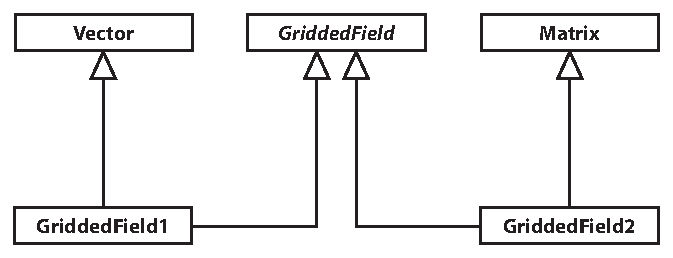
\includegraphics{Figs/development/griddedfields_inheritance}
\caption{UML diagram of gridded field inheritance.}
\zlabel{fig:griddedfields:uml}
\end{center}
\end{figure}


\section{Constructing Gridded Fields}
%-------------------------------------------------------------------------
\zlabel{sec:griddedfields:construct}


\subsection{Creation}
%-------------------------------------------------------------------------
\zlabel{sec:griddedfields:create}

Each \artsstyle{GriddedFieldX} offers two constructors. One default constructor that creates an unnamed gridded field and a second constructor that takes a String with the name of the gridded field as an argument.

\begin{verbatim}
  GriddedField1 gfone("I'm a GriddedField1");
  GriddedField2 gftwo;
  
  gftwo.set_name ("I'm a GriddedField2");
\end{verbatim}


\subsection{Initializing the grids}
%-------------------------------------------------------------------------
\zlabel{sec:griddedfields:initgrids}

Once a gridded field has been created, we can start setting up the grids. There are two different types of grids, a numeric grid and a string grid.

\begin{verbatim}
Vector gfonegrid(1,5,1);        // gfonegrid = [1,2,3,4,5]
gfone.set_grid(0, gfonegrid);   // Set grid for the vector elements

MakeArray<String> gftwogrid0("Channel 1", "Channel2", "Channel3");
Vector gftwogrid1(1,5,1);       // gftwogrid1 = [1,2,3,4,5]

gftwo.set_grid(0, gftwogrid0);  // Set grid for the matrix rows
gftwo.set_grid(1, gftwogrid1);  // Set grid for the matrix columns
\end{verbatim}

Note that the first grid corresponds to the highest dimension of the data. This means grid 0 in a \artsstyle{GriddedField2} corresponds to the rows of the matrix. Grid 1 corresponds to the columns.

In addition to the grid values, a name can be assigned to each grid.

\begin{verbatim}
gfone.set_grid_name (0, "Pressure");

gftwo.set_grid_name (0, "Instrument channel");
gftwo.set_grid_name (1, "Pressure");
\end{verbatim}

\subsection{Initializing the data}
%-------------------------------------------------------------------------
\zlabel{sec:griddedfields:initdata}

Because gridded fields do not only inherit from \artsstyle{GriddedField} but also from the class of the data they contain, it is possible to treat them in exactly the same way. See Figure \zref{fig:griddedfields:objects}.

\begin{figure}[ht!]
\begin{center}
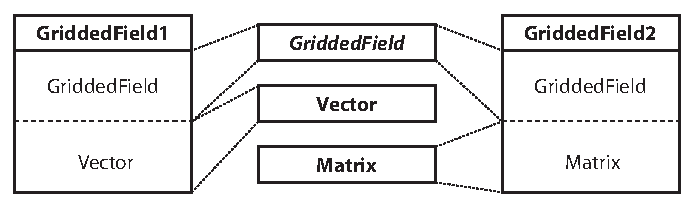
\includegraphics{Figs/development/griddedfields_objects}
\caption{Visualization of gridded field objects.}
\zlabel{fig:griddedfields:objects}
\end{center}
\end{figure}

Let us take the \artsstyle{gfone} variable from the previous examples. \artsstyle{gfone} is a \artsstyle{GriddedField1} which means it has \artsstyle{GriddedField} and \artsstyle{Vector} as superclasses. Polymorphism allows us to use a \artsstyle{GriddedField1} in every place where it is valid to use a \artsstyle{Vector}. The only requirement is to cast the gridded field to the corresponding data type.

\begin{verbatim}
Vector avector(1,5,0.5);    // avector = [1,1.5,2,2.5,3]

(Vector&)gfone = avector;

Matrix amatrix(2,3,4.);     // amatrix = [[4,4,4],[4,4,4]]

(Matrix&)gftwo = amatrix;
\end{verbatim}

\subsection{Consistency check}
%-------------------------------------------------------------------------
\zlabel{sec:griddedfields:consistency}

After initializing or changing either the grids or the data, it can happen that the size of the grids does not match up with the size of the data anymore. Each gridded field provides a convenience function which can be called to make a consistency check.

\begin{verbatim}
if (!gfone.checksize())
  cout << gfone.get_name()
       << ": Sizes of grid and data don't match" << endl;

// This should fail!
if (!gftwo.checksize())
  cout << gftwo.get_name()
       << ": Sizes of grids and data don't match" << endl;
\end{verbatim}

%%% Local Variables:
%%% mode: latex
%%% TeX-master: "arts_developer"
%%% End:


%
% To start the document, use
%  \levela{...}
% For lover level, sections use
%  \levelb{...}
%  \levelc{...}
%
\levela{Interpolation}
%-------------------------------------------------------------------------
\label{sec:interpolation}


%
% Document history, format:
%  \starthistory
%    date1 & text .... \\
%    date2 & text .... \\
%    ....
%  \stophistory
%
\starthistory
  020528 & Created by Stefan Buehler.\\
\stophistory




%
% Introduction
%

There are no general single-step interpolation functions in ARTS.
Instead, there is a set of useful utility functions that can be used
to achieve interpolation. Roughly, you can separate these into
functions determining grid position arrays, functions determining
interpolation weight tensors, and functions applying the
interpolation. Doing an interpolation thus requires a chain of
function calls:
\begin{enumerate}
\item \verb|gridpos| (one for each interpolation dimension)
\item \verb|interpweights|
\item \verb|interp|
\end{enumerate}
Currently implemented in ARTS is mulitlinear interpolation in up to 6
dimensions. (Is the 6D case called hexa-linear interpolation?)  The
necessary functions and their interaction will be explained in this
chapter.

\levelb{Implementation files}
%-------------------------------------------------------------------------

Variables and functions related to interpolation are defined in the files:
\begin{itemize}
\item \verb|interpolation.h|
\item \verb|interpolation.cc|
\item \verb|test_interpolation.cc|
\end{itemize}
The first two files contain the declarations and implementation, the
last file some usage examples.

\levelb{Green and blue interpolation}
%-------------------------------------------------------------------------

\begin{figure}[htbp]
  \centering
  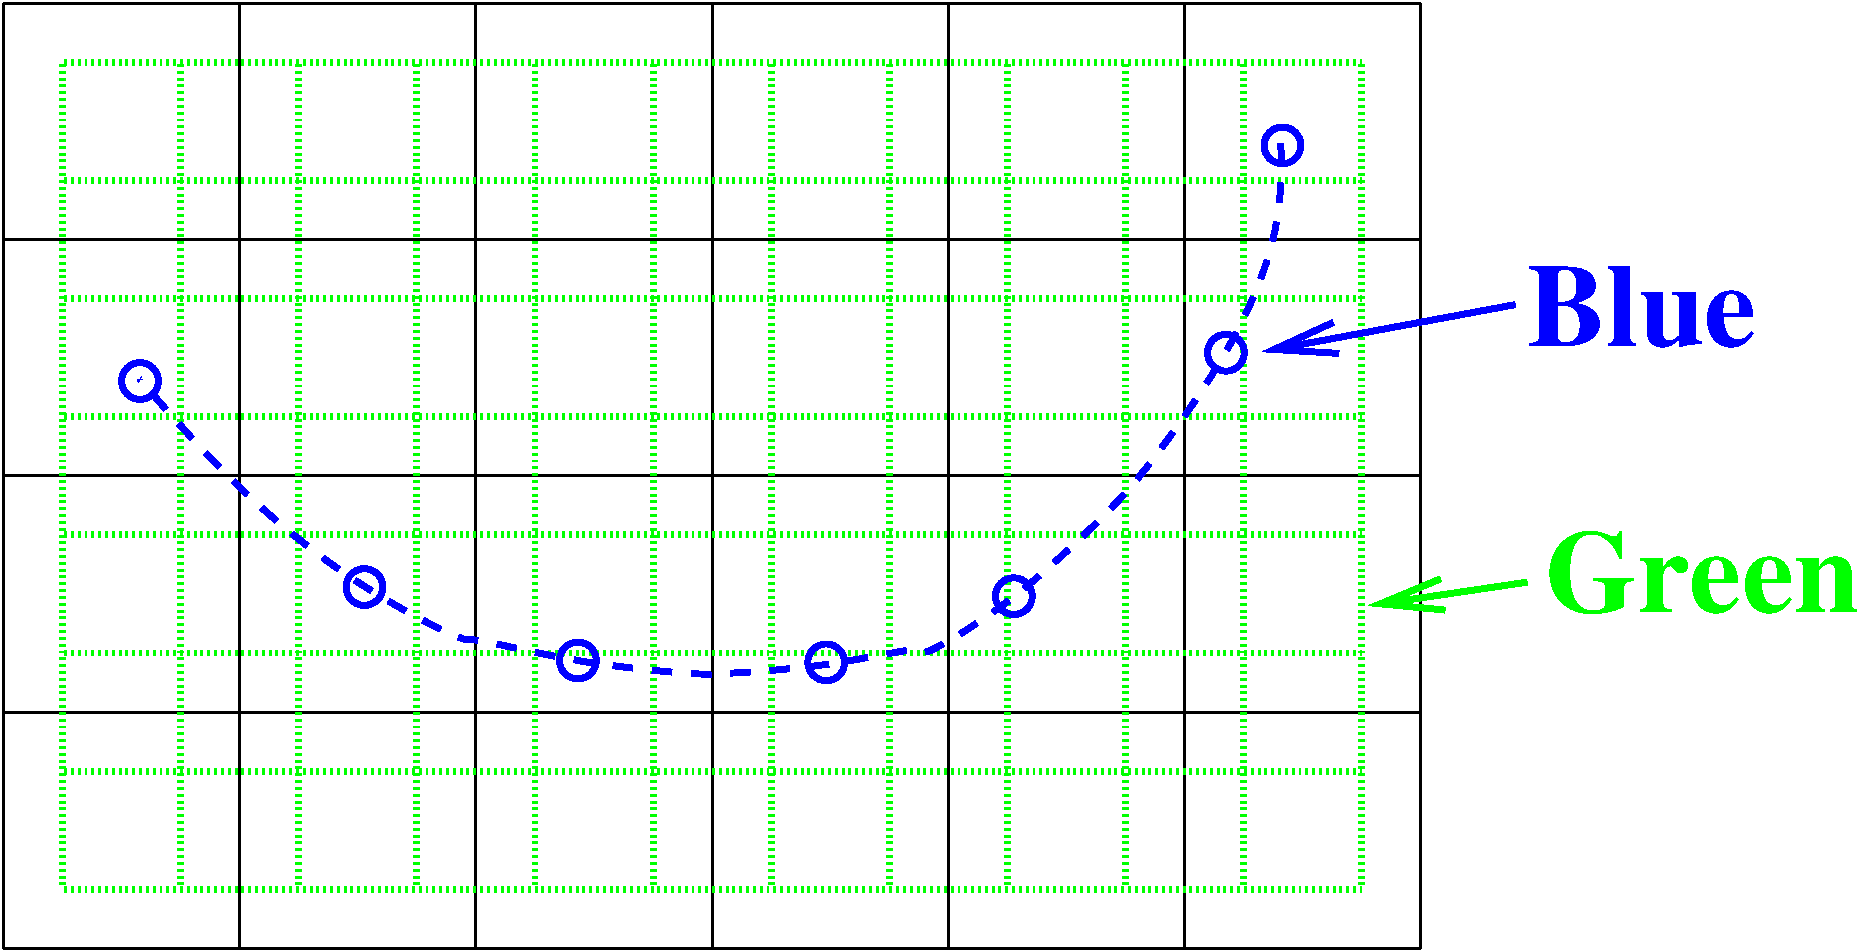
\includegraphics[width=.6\hsize]{interpolation/interpolation_types}
  \caption{The two different types of interpolation. Green (dotted):
    Interpolation to a new grid, output has same dimension as input,
    in this case 2D. Blue (dashed): Interpolation to a sequence of
    points, output is always 1D.}
  \label{fig:interpolation:types}
\end{figure}

There are two different types of interpolation in ARTS:
\begin{description}
\item[Green Interpolation:] Interpolation of a gridded field to a new
  grid.
\item[Blue Interpolation:] Interpolation of a gridded field to a
  sequence of positions.
\end{description}
Figure \ref{fig:interpolation:types} illustrates the different types
for a 2D example. 

The first step of an interpolation always consists in determining
where your new points are, relative to the original grid. You can do
this separately for each dimension. The positions have to be stored
somehow, which is described in the next section.



\levelb{Grid positions}
%-------------------------------------------------------------------------

A grid position specifies where an interpolation point is, relative
to the original grid. It consists of three parts, an \verb|Index| giving the
original grid index below the interpolation point, a \verb|Numeric|
giving the fractional distance to the next original grid point, and a
\verb|Numeric| giving 1 minus this number. Of course, the last element is
redundant. However, it is efficient to store this, since it is used
many times over. We store the two numerics in a plain C array of
dimension 2. (No need to use a fancy Array or Vector for this, since
the dimension is fixed.) So the structure is:

\begin{verbatim}
struct GridPos {
   Index   idx;      /*!< Original grid index below
                          interpolation point. */
   Numeric fd[2];    /*!< Fractional distance to next point
                          (0<=fd[0]<=1), fd[1] = 1-fd[0]. */ 
};
\end{verbatim}

For example, \verb|idx|=3 and \verb|fd|=0.5 means that this interpolation point is
half-way between index 3 and 4 of the original grid.  Note, that
`below' in the first paragraph means `with a lower index'. If the
original grid is sorted in descending order, the value at the grid
point below the interpolation point will be numerically higher than
the interpolation point.  In other words, grid positions and
fractional distances are defined relative to the order of the original
grid. Examples:

{\small
\begin{verbatim}
old grid = 2 3
new grid = 2.25
idx      = 0
fd[0]    = 0.25

old grid = 3 2
new grid = 2.25
idx      = 0
fd[0]    = 0.75
\end{verbatim}
}

Note that \verb|fd[0]| is different in the second case, because the old grid
is sorted in descending order. Note also that \verb|idx| is the same in
both cases.

Grid positions for a whole new grid are stored in an \verb|Array<GridPos>|
(called \verb|ArrayOfGridPos|). 

\levelb{Setting up grid position arrays}
%----------------------------------------------------------------------

There is only one function to set up grid position arrays:

{\small
\begin{verbatim}
void gridpos( ArrayOfGridPos& gp,
              ConstVectorView old_grid,
              ConstVectorView new_grid );
\end{verbatim}
}

\hspace{-\parindent}Some points to remember:
\begin{itemize}
\item As usual, the output \verb|gp| has to have the right dimension. 
  
\item The old grid has to be strictly sorted. It can be in ascending
  or descending order. But there must not be any duplicate values.
  Furthermore, the old grid must contain at least two points.
  
\item   The new grid does not have to be sorted, but the function will be
  faster if it is sorted or mostly sorted. It is ok if the new grid
  contains only one point.
  
\item   The beauty is, that this is all it needs to do also interpolation in
  higher dimensions: You just have to call gridpos for all the
  dimensions that you want to interpolate.
  
\item   Note also, that for this step you do not need the field itself at
  all!
\end{itemize}

\levelb{Interpolation weights}
%----------------------------------------------------------------------

As explained in the `Numerical Recipes'
\citep{numerical_recipes_C:97}, 2D bi-linear interpolation means, that
the interpolated value is a weighted average of the original field at
the four corner points of the grid square in which the interpolation
point is located. For simplicity, we label the four corner points
counterclockwise, starting from the lower left point (Figure
\ref{fig:interpolation:square}).  Then the interpolated value is given
by:
\begin{eqnarray}
  y(t,u)
  &=& (1-t)*(1-u)*y_1 \nonumber \\
  & & \mbox{} + t*(1-u)*y_2 \nonumber \\
  & & \mbox{} + t*u*y_3 \nonumber \\
  & & \mbox{} + (1-t)*u*y_4 \nonumber \\
  &=& w_1*y_1 + w_2*y_2 + w_3*y_3 + w_4*y_4
\label{eq:interpolation:weights}
\end{eqnarray}
where $t$ and $u$ are the fractional distances between the
corner points in the two dimensions, $y_i$ are the field values
at the corner points, and $w_i$ are the interpolation weights.

\begin{figure}
  \centering
  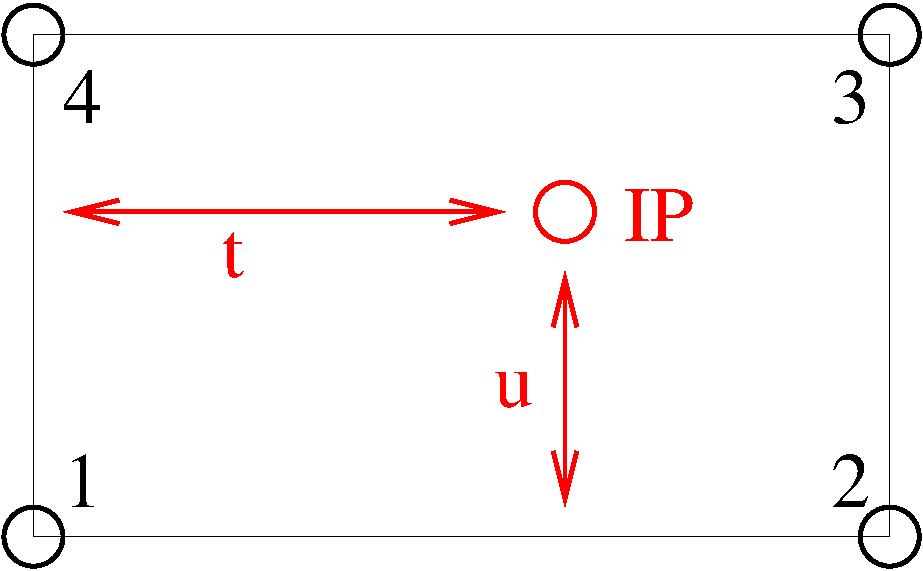
\includegraphics[width=.4\hsize]{interpolation/interpolation_square}
  \caption{The grid square for 2D interpolation. The numbers 1\ldots 4
    mark the corner points, IP is the interpolation point, $t$ and $u$
    are the fractional distances in the two dimensions.}
  \label{fig:interpolation:square}
\end{figure}

(By the way, I have discovered that this is exactly the result that
you get if you first interpolate linearly in one dimension, then in
the other. I was playing around with this a bit, but it is the more
efficient way to pre-calculate the $w_i$ and do all dimensions at once.

How many interpolation weights one needs for a multilinear
interpolation depends on the dimension of the interpolation: There are
exactly $2^n$ interpolation weights for an $n$ dimensional
interpolation.  These weights have have to be computed for each
interpolation point (each grid point of the new grid, if we do a
`green' type interpolation. Or each point in the sequence, if we do a
`blue' type interpolation).

This means, calculating the interpolation weights is not exactly
cheap, especially if one interpolates simultaneously in many
dimensions. On the other hand, one can save a lot by re-using the
weights.  Therefore, interpolation weights in ARTS are stored in a
tensor which has one more dimension than the output field. The last
dimension is for the weight, so this last dimension has the extent 4
in the 2D case, 8 in the 3D case, and so on (always $2^n$).

In the case of a `blue' type interpolation, the weights are
always stored in a matrix, since the output field is always 1D (a
vector). 

\levelb{Setting up interpolation weight tensors}
%----------------------------------------------------------------------

Interpolation weight tensors can be computed by a family of functions,
which are all called \verb|interpweights|. Which function is actually
used depends on the dimension of the input and output quantities. For
this step we still do not need the actual fields, just the grid
positions.

\levelc{Blue interpolation}

In this case the functions are:

{\small
\begin{verbatim}
void interpweights( MatrixView itw,
                    const ArrayOfGridPos& cgp );
void interpweights( MatrixView itw,
                    const ArrayOfGridPos& rgp,
                    const ArrayOfGridPos& cgp );
void interpweights( MatrixView itw,
                    const ArrayOfGridPos& pgp,
                    const ArrayOfGridPos& rgp,
                    const ArrayOfGridPos& cgp );
void interpweights( MatrixView itw,
                    const ArrayOfGridPos& vgp,
                    const ArrayOfGridPos& sgp,
                    const ArrayOfGridPos& bgp,
                    const ArrayOfGridPos& pgp,
                    const ArrayOfGridPos& rgp,
                    const ArrayOfGridPos& cgp );
\end{verbatim}
}

In all cases, the dimension of \verb|itw| must be consistent with the
given grid position arrays and the dimension of the interpolation
(last dimension $2^n$). Because the grid position arrays are
interpreted as defining a sequence of positions they must all have
the same length.

\levelc{Green interpolation}

In this case the functions are:

{\small
\begin{verbatim}
void interpweights( Tensor3View itw,
                    const ArrayOfGridPos& rgp,
                    const ArrayOfGridPos& cgp );
void interpweights( Tensor4View itw,
                    const ArrayOfGridPos& pgp,
                    const ArrayOfGridPos& rgp,
                    const ArrayOfGridPos& cgp );
void interpweights( Tensor5View itw,
                    const ArrayOfGridPos& bgp,
                    const ArrayOfGridPos& pgp,
                    const ArrayOfGridPos& rgp,
                    const ArrayOfGridPos& cgp );
void interpweights( Tensor6View itw,
                    const ArrayOfGridPos& sgp,
                    const ArrayOfGridPos& bgp,
                    const ArrayOfGridPos& pgp,
                    const ArrayOfGridPos& rgp,
                    const ArrayOfGridPos& cgp );
void interpweights( Tensor7View itw,
                    const ArrayOfGridPos& vgp,
                    const ArrayOfGridPos& sgp,
                    const ArrayOfGridPos& bgp,
                    const ArrayOfGridPos& pgp,
                    const ArrayOfGridPos& rgp,
                    const ArrayOfGridPos& cgp );
\end{verbatim}
}

In this case the grid position arrays are interpreted as defining the
grids for the interpolated field, therefore they can have different
lengths. Of course, \verb|itw| must be consistent with the length of
all the grid position arrays, and with the dimension of the
interpolation (last dimension $2^n$).

\levelb{The actual interpolation}
%----------------------------------------------------------------------

For this final step we need the grid positions, the
interpolation weights, and the actual fields. For each interpolated
value, the weights are applied to the appropriate original field values
and the sum is taken (see Equation
\ref{eq:interpolation:weights}). The \verb|interp| family of functions
performs this step.

\levelc{Blue interpolation}

{\small
\begin{verbatim}
void interp( VectorView            ia,
             ConstMatrixView       itw,
             ConstVectorView       a,    
             const ArrayOfGridPos& cgp);
void interp( VectorView            ia,
             ConstMatrixView       itw,
             ConstMatrixView       a,    
             const ArrayOfGridPos& rgp,
             const ArrayOfGridPos& cgp);
void interp( VectorView            ia,
             ConstMatrixView       itw,
             ConstTensor3View      a,    
             const ArrayOfGridPos& pgp,
             const ArrayOfGridPos& rgp,
             const ArrayOfGridPos& cgp);
void interp( VectorView            ia,
             ConstMatrixView       itw,
             ConstTensor4View      a,    
             const ArrayOfGridPos& bgp,
             const ArrayOfGridPos& pgp,
             const ArrayOfGridPos& rgp,
             const ArrayOfGridPos& cgp);
void interp( VectorView            ia,
             ConstMatrixView       itw,
             ConstTensor5View      a,    
             const ArrayOfGridPos& sgp,
             const ArrayOfGridPos& bgp,
             const ArrayOfGridPos& pgp,
             const ArrayOfGridPos& rgp,
             const ArrayOfGridPos& cgp);
void interp( VectorView            ia,
             ConstMatrixView       itw,
             ConstTensor6View      a,    
             const ArrayOfGridPos& vgp,
             const ArrayOfGridPos& sgp,
             const ArrayOfGridPos& bgp,
             const ArrayOfGridPos& pgp,
             const ArrayOfGridPos& rgp,
             const ArrayOfGridPos& cgp);
\end{verbatim}
}

\levelc{Green interpolation}

{\small
\begin{verbatim}
void interp( MatrixView            ia,
             ConstTensor3View      itw,
             ConstMatrixView       a,   
             const ArrayOfGridPos& rgp,
             const ArrayOfGridPos& cgp);
void interp( Tensor3View           ia,
             ConstTensor4View      itw,
             ConstTensor3View      a,   
             const ArrayOfGridPos& pgp,
             const ArrayOfGridPos& rgp,
             const ArrayOfGridPos& cgp);
void interp( Tensor4View           ia,
             ConstTensor5View      itw,
             ConstTensor4View      a,   
             const ArrayOfGridPos& bgp,
             const ArrayOfGridPos& pgp,
             const ArrayOfGridPos& rgp,
             const ArrayOfGridPos& cgp);
void interp( Tensor5View           ia,
             ConstTensor6View      itw,
             ConstTensor5View      a,   
             const ArrayOfGridPos& sgp,
             const ArrayOfGridPos& bgp,
             const ArrayOfGridPos& pgp,
             const ArrayOfGridPos& rgp,
             const ArrayOfGridPos& cgp);
void interp( Tensor6View           ia,
             ConstTensor7View      itw,
             ConstTensor6View      a,   
             const ArrayOfGridPos& vgp,
             const ArrayOfGridPos& sgp,
             const ArrayOfGridPos& bgp,
             const ArrayOfGridPos& pgp,
             const ArrayOfGridPos& rgp,
             const ArrayOfGridPos& cgp);
\end{verbatim}
}

\levelb{Examples}
%----------------------------------------------------------------------

\levelc{A simple example}

This example is contained in file \verb|test_interpolation.cc|.

{\small
\begin{verbatim}
void test05()
{
  cout << "Very simple interpolation case\n";

  Vector og(1,5,+1);            // 1, 2, 3, 4, 5
  Vector ng(2,5,0.25);          // 2.0, 2,25, 2.5, 2.75, 3.0

  cout << "Original grid:\n" << og << "\n";
  cout << "New grid:\n" << ng << "\n";

  // To store the grid positions:
  ArrayOfGridPos gp(ng.nelem());

  gridpos(gp,og,ng);
  cout << "Grid positions:\n" << gp;

  // To store interpolation weights:
  Matrix itw(gp.nelem(),2);
  interpweights(itw,gp);
    
  cout << "Interpolation weights:\n" << itw << "\n";

  // Original field:
  Vector of(og.nelem(),0);
  of[2] = 10;                   // 0, 0, 10, 0, 0

  cout << "Original field:\n" << of << "\n";

  // Interpolated field:
  Vector nf(ng.nelem());

  interp(nf, itw, of, gp);

  cout << "New field:\n" << nf << "\n";
}
\end{verbatim}
}

\hspace{-\parindent}Ok, maybe you think this is not so simple, but a
large part of the code is either setting up the example grids and
fields, or output. And here is how the output looks like:

{\small
\begin{verbatim}
Very simple interpolation case
Original grid:
  1   2   3   4   5
New grid:
  2 2.25 2.5 2.75   3
Grid positions:
   1 0    1
   1 0.25 0.75
   1 0.5  0.5
   1 0.75 0.25
   1 1    0
Interpolation weights:
  1   0
0.75 0.25
0.5 0.5
0.25 0.75
  0   1
Original field:
  0   0  10   0   0
New field:
  0 2.5   5 7.5  10
\end{verbatim}
}

\levelc{A more elaborate example}

What if you want to interpolate only some dimensions of a tensor,
while retaining others? --- You have to make a loop yourself, but it
is very easy. Below is an explicit example for a more complicated
interpolation case. (Green type interpolation of all pages of a
Tensor3.) This example is also contained in file
\verb|test_interpolation.cc|.

{\small
\begin{verbatim}
void test04()
{
  cout << "Green type interpolation of all "
       << "pages of a Tensor3\n";

  // The original Tensor is called a, the new one n. 

  // 10 pages, 20 rows, 30 columns, all grids are: 1,2,3
  Vector  a_pgrid(1,3,1), a_rgrid(1,3,1), a_cgrid(1,3,1); 
  Tensor3 a( a_pgrid.nelem(),
             a_rgrid.nelem(),
             a_cgrid.nelem() ); 
  a = 0;
  // Put some simple numbers in the middle of each page:
  a(0,1,1) = 10;
  a(1,1,1) = 20;
  a(2,1,1) = 30;

  // New row and column grids:
  // 1, 1.5, 2, 2.5, 3
  Vector  n_rgrid(1,5,.5), n_cgrid(1,5,.5); 
  Tensor3 n( a_pgrid.nelem(),
             n_rgrid.nelem(),
             n_cgrid.nelem() ); 

  // So, n has the same number of pages as a, 
  // but more rows and columns.

  // Get the grid position arrays:
  ArrayOfGridPos n_rgp(n_rgrid.nelem()); // For rows.
  ArrayOfGridPos n_cgp(n_cgrid.nelem()); // For columns.

  gridpos( n_rgp, a_rgrid, n_rgrid );
  gridpos( n_cgp, a_cgrid, n_cgrid );

  // Get the interpolation weights:
  Tensor3 itw( n_rgrid.nelem(), n_cgrid.nelem(), 4 );
  interpweights( itw, n_rgp, n_cgp );

  // Do a "green" interpolation for all pages of a:

  for ( Index i=0; i<a.npages(); ++i )
    {
      // Select the current page of both a and n:
      ConstMatrixView ap = a( i,
                              Range(joker), Range(joker) );
      MatrixView      np = n( i,
                              Range(joker), Range(joker) );

      // Do the interpolation:
      interp( np, itw, ap, n_rgp, n_cgp );

      // Note that this is efficient, because interpolation
      // weights and grid positions are re-used.
    }

  cout << "Original field:\n";
  for ( Index i=0; i<a.npages(); ++i )
      cout << "page " << i << ":\n"
           << a(i,Range(joker),Range(joker)) << "\n";

  cout << "Interpolated field:\n";
  for ( Index i=0; i<n.npages(); ++i )
      cout << "page " << i << ":\n"
           << n(i,Range(joker),Range(joker)) << "\n";
}
\end{verbatim}
}

\hspace{-\parindent}The output is:

{\small
\begin{verbatim}
Green type interpolation of all pages of a Tensor3
Original field:
page 0:
  0   0   0
  0  10   0
  0   0   0
page 1:
  0   0   0
  0  20   0
  0   0   0
page 2:
  0   0   0
  0  30   0
  0   0   0
Interpolated field:
page 0:
  0   0   0   0   0
  0 2.5   5 2.5   0
  0   5  10   5   0
  0 2.5   5 2.5   0
  0   0   0   0   0
page 1:
  0   0   0   0   0
  0   5  10   5   0
  0  10  20  10   0
  0   5  10   5   0
  0   0   0   0   0
page 2:
  0   0   0   0   0
  0 7.5  15 7.5   0
  0  15  30  15   0
  0 7.5  15 7.5   0
  0   0   0   0   0
\end{verbatim}
}

\levelb{Summary}
%----------------------------------------------------------------------

Now you probably understand better what was written at the very
beginning of this chapter, namely that doing an interpolation always
requires the chain of function calls:
\begin{enumerate}
\item \verb|gridpos| (one for each interpolation dimension)
\item \verb|interpweights|
\item \verb|interp|
\end{enumerate}
If you are interested in how the functions really work, look in file
\verb|interpolation.cc|. The documentation there is quite detailed.
When you are using interpolation, you should always give some thought
to whether you can re-use grid positions or even interpolation
weights. This can really save you a lot of computation time. For
example, if you want to interpolate several fields --- which are all
on the same grids --- to some position, you only have to compute the
weights once.


%%% Local Variables: 
%%% mode: latex 
%%% TeX-master: "uguide" 
%%% TeX-master: "uguide"
%%% End:


\chapter{Integration functions}
%--------------------------------------------------------------------------
\label{sec:integration}

\starthistory
  220802 & Created and written by Sreerekha T.R.\\
  220103 & Included mathematical description for implemented integration method(CE).\\
\stophistory

%
% Introduction
%
A radiative transfer model which takes into account the effect of
scattering involves integration of certain quantities over the angles
of observation.  For example from Section
\ref{sec:scattering:solution_rte} it is clear that computing  
scattering cross-section  and scattering integral term requires
integration over zenith and azimuth directions. There are a wide range of
methods that can be used for numerical integration. They can be used
depending on various factors starting from how accurate the result
should be to the behaviour of the function. The one which is
implemented in ARTS is the trapezoidal integration method. 


\section{Implementation files}
%-------------------------------------------------------------------------
\label{sec:integration:files}

The integration functions can be found in the files:
\begin{itemize}
\item \artsstyle{math\_funcs.h}
\item \artsstyle{math\_funcs.cc}
\end{itemize}
The implementation function \artsstyle {AngIntegrate\_trapezoid}is
discussed in the second file. 

\section{Trapezoidal Integration}
%------------------------------------------------------------------------
\label{sec:integration:trapezoidal}

Trapezoidal Integration method comes under the Newton-Cotes formulas
where integration of a function is approximated by the area under the
curve described by the function.  Trapezoidal integration assumes that
the area under the curve is trapezoid.  

Trapezoidal rule : 
\begin{eqnarray}
\label{eq:trapezoidal_rule}
{\int_{x_1}^{x_2} f(x)dx}  = \frac{1}{2} h (f_1 + f_2) + O(h^3 f^{''})
\end{eqnarray}
This is a two-point formula ($x_1$ and $x_2$).  It is exact for
polynomials upto and including degree 1, i.e., f(x) = x. $O(h^3
f^{''})$ signifies how far is the true answer from the estimate. 

If we use eq. \ref{eq:trapezoidal_rule} $N - 1$ times, to do the
integration in the intervals $(x_1, x_2)$,  $(x_2, x_3)$, ...,
$(x_{N-1}, x_N)$, and then add the results, we obtain extended formula
for the integral from $x_1$ to $x_N$.

Extended Trapezoidal rule :
\begin{eqnarray}
\label{eq:ext_trapezoidal_rule}
{\int_{x_1}^{x_N} f(x)dx}  = \frac{1}{2} h \left [f_1 + 2(f_2 + f_3 +
... +f_{N-1})+f_N \right] + O\left [ \frac {(b-a)^3 f^{''}}{N^2} \right]
\end{eqnarray}

The last term tells how much the error will be decreased by taking
more number of steps. 

\section{Solid Angle Integration}
%------------------------------------------------------------------------
\label{sec:integration:solid_angle}
In our scattering problem, we are often encountered with a double integration
of functions over zenith and azimuth angles (see Chapter
\ref{sec:scattering}).  One way to achieve
double integration is to use repeated
one-dimensional trapezoidal integration.  This is effective of course
only if the boundary is simple and the function is very smooth.  If
the function is strongly peaked and if know where it occurs, integral
should be broken into smaller regions so that the 
integrand is smooth in each.  Another thing is to take into account
the symmetry of the function as well as the boundary. For example in
our case, if the radiation is symmetric about the azimuth, the
integration in that direction returns constant value of $2 \pi$ and we
need to do only integration over zenith directions.  

The general form of a solid angle integration is
\begin{equation}
  \label{eq:solid_int}
S = \int_{4\pi} f(\omega) \DiffD\omega
\end{equation}
In spherical coordinates we can write:
\begin{equation}
  \label{eq:sol_int_sph}
 S = \int_0^\pi \int_0^{2\pi} f(\theta,\phi) \sin\theta \quad\DiffD\theta\DiffD\phi
\end{equation}
A double integration can be splitted into two single integrations:
\begin{eqnarray}
 S &=& \int_0^\pi \left(\int_0^{2\pi}  f(\theta,\phi) \sin\theta \DiffD\phi \right) \DiffD\theta \\
 &=& \int_0^\pi g(\theta) \DiffD\theta
\end{eqnarray}
If we have to integrate a vector, we can apply this method componentwise.

To solve the integral numerically we discretize $\theta$ and $\phi$ and obtain two angular grids ( $[\theta_0, \theta_1, \cdots, \theta_n]$  and $[\phi_0, \phi_1, \cdots, \phi_m]$). 
Then we can first calculate $g(\theta_j)$ for all $\theta_j$ unsing the trapezoidal method.
\begin{equation}
  g(\theta_j) = \sum_{i=1}^m \sin\theta_j \frac{f(\theta_j, \phi_i) + f(\theta_j, \phi_{i+1})}{2} \cdot (\phi_{i+1} - \phi_i)  
\end{equation}
The final step is to sum up all $g(\theta_j)$, again applying the trapezoidal method.
\begin{equation}
  S = \sum_{j=1}^n \frac{g(\theta_j) + g(\theta_{j+1})}{2} \cdot  (\theta_{j+1} - \theta_j)  
\end{equation}

If the radiation is symmetric about the azimuth we just calculate:
\begin{equation}
  S_{sym} = 2\pi \int_0^{\pi} f(\theta) \sin(\theta) \DiffD \theta 
\end{equation}
Unsing the trapezoidal method this can be written as:
\begin{equation}
  S_{sym} =  2\pi \sum_{j=1}^n \frac{h(\theta_j) + h(\theta_{j+1})}{2} \cdot  (\theta_{j+1} - \theta_j)  
\end{equation}
where $h(\theta) = \sin\theta\cdot f(\theta)$.
 
\vspace{2ex}



The function  \artsstyle{AngIntegrate\_trapezoid} takes as input the integrand and the angles over which
the integration has to be done. For example in this case it can be the
zenith and azimuth angle
grid.
\begin{verbatim}  
Numeric AngIntegrate_trapezoid(MatrixView Integrand,
                               ConstVectorView za_grid,
                               ConstVectorView aa_grid)
\end{verbatim}
The integrand has the same number of rows as zenith angle grid
and columns as azimuth angle grid.  The inner loop does trapezoidal
integration of the integrand over all azimuth angles and the result is
stored in a Vector  res1[i]. Note that the integrand at every point
has to be multiplied with \artsstyle {sin (za\_grid[i] * DEG2RAD)}
since we are integrating over solid angles.  The outer loop 
does an integration of res1[i] over all zentih angles.  The result of
this is returned back to the calling function.  


%%% Local Variables: 
%%% mode: latex
%%% TeX-master: t
%%% End: 

\levela{Linear Algebra functions}
%--------------------------------------------------------------------------
\label{sec:lin_alg}

\starthistory
  020502 & Created and written by Claudia Emde.\\
\stophistory

%
% Introduction
%

Solving the vector radiative transfer equation requires the
computation of linear equation systems and the matrix
exponential. This section describes the functions which are implemented
in ARTS and it gives instructions how these functions can be used, also
for other purposes than the radiative transfer calculations.

\levelb{Implementation files}
%-------------------------------------------------------------------------
\label{sec:lin_alg:files}

All the functions described below can be found in the files:
\begin{itemize}
\item \artsstyle{lin\_alg.h}
\item \artsstyle{lin\_alg.cc}
\end{itemize}
The template class \artsstyle{Array} and the classes \artsstyle{Matrix} and
\artsstyle{Vector} are used, therefore the linear algebra functions require
the files:
\begin{itemize}
\item \artsstyle{matpackI.h}
\item \artsstyle{make\_vector.h}
\item \artsstyle{array.h}
\item \artsstyle{matpackI.cc}
\item \artsstyle{make\_vector.cc}
\item \artsstyle{array.cc}
\end{itemize}
Furthermore logical functions contained in
\begin{itemize}
\item \artsstyle{logic.h}
\item \artsstyle{logic.cc}
\end{itemize}
are used to check the dimensions of input matrices for various functions.


\levelb{Linear Equation Systems}
%------------------------------------------------------------------------
\label{sec:lin_alg:lineqsys}


For solving a set of linear equations 
\begin{eqnarray}
\label{eq:lin_equ_sys}
{\bf A} {\bf x} = {\bf b}
\end{eqnarray}
the LU decomposition method is implemented.A slightly modified version
of the algorithm described in
[\cite{numerical_recipes_C:97}] is used here. An alternative method
is the Gauss-Jordan elimination, but this method is three times
slower than the LU decomposition method
[\cite{numerical_recipes_C:97}, p.36]. The LU decomposition method
reqires two functions, \artsstyle{ludcmp} and \artsstyle{lubacksub},
which will be decribed below.
\vspace{0.5cm}\\
The following example for a three dimensional equation sytem 
demonstrates how to solve a linear
equation sytem of the type
(\ref{eq:lin_equ_sys}):
\begin{itemize}
\item Create matrix A, vector b: \\
  \artsstyle{A = Matrix(3,3);} \\
  \artsstyle{A(1,1) = 4;}\\
  \artsstyle{A(2,1) = 3;}\\
  $\cdots$\\
  \artsstyle{b = Vector(3);}\\
  \artsstyle{b(1) = 7;}\\
  $\cdots$
\item Initialize solution vector x and two other variables needed for
  storing intermediate results:\\
  \artsstyle{x = Vector(3);}\\
  \artsstyle{LU = Matrix(3,3);}\\
  \artsstyle{indx = ArrayOfIndex(3);}
\item Call LU decomposition function (see Section \ref{sec:lin_alg:lu_decomp}): \\
  \artsstyle{ludcmp(LU, indx, A);}
\item Call LU backsubstitution function (see Section \ref{sec:lin_alg:backsub}): \\
  \artsstyle{lubacksub(x, LU, b, indx);}
\item Print the solution vector:\\
  \artsstyle{cout << x;}
\end{itemize}

\levelc{LU Decomposition}
%------------------------------------------------------------------------
\label{sec:lin_alg:lu_decomp}

A LU decomposition is a procedure for decomposing a square matrix {\bf
  A} with
dimension $n$ into a product of a lower triangular matrix {\bf L} (has
elements only on the diagonal elements and below) and
an upper triangular matrix {\bf U} (has elements only on the diagonal
and above):
\begin{equation}
  \label{eq:lu_decomp}
  {\bf L}\cdot{\bf U} ={\bf A} 
\end{equation}
For a 3 x 3 matrix equation \ref{eq:lu_decomp} would look like this: 
\[ \left(
  \begin{array}{ccc}
    l_{11} & 0 & 0 \\
    l_{21} & l_{22} & 0 \\
    l_{31} & l_{32} & l_{33}
    \end{array} \right)
\cdot
\left(
  \begin{array}{ccc}
    u{11} & u_{12} & u_{13} \\
    0 & u_{22} & u_{23}\\
    0 & 0 & u_{33}
    \end{array} \right)
=
\left(
  \begin{array}{ccc}
    a_{11} & a_{12} & a_{13} \\
    a_{21} & a_{22} & a_{23} \\
    a_{31} & a_{32} & a_{33}
    \end{array} \right)
\]
The decomposition can be used to rewrite the linear set of equations
(\ref{eq:lin_equ_sys}) in the following way:
\begin{eqnarray}
  {\bf A}\cdot{\bf x} = ({\bf L}\cdot{\bf U})\cdot{\bf x} = {\bf
    L}\cdot({\bf U}\cdot{\bf x}) = {\bf b}
\end{eqnarray}
First 
\begin{equation}
  {\bf L} \cdot{\bf y} = {\bf b}
\end{equation}
is solved for the vector ${\bf y}$ which can be done by
forward substitution (see section \ref{sec:lin_alg:backsub}). Then 
\begin{equation}
  {\bf U} \cdot{\bf x} = {\bf y}
\end{equation}
is solved again by backsubstitution. 
The advantage in breaking up one linear set into two successive ones
is that the solution of a triangular set of equations is quite trivial.

The function \artsstyle{ludcmp} requires a square matrix of arbitrary
dimension $n$ as input and performs the LU decomposition. It returns one
matrix which contains both matrices, ${\bf L}$ and ${\bf U}$. 
For the lower triangular matrix  ${\bf L}$ the diagonal elements 
are chosen to be 1, then the other elements of ${\bf L}$ and ${\bf U}$
are determined. This is possible, as the LU decomposition is an under
determined equation sytem with $n^2$ equations for $n^2+n$ unknowns. 
The output matrix does not include the diagonal of ${\bf L}$, in the
three-dimensional case it has the following elements:
\[ \left(
  \begin{array}{ccc}
    u_{11} & u_{12} & u_{13} \\
    l_{21} & u_{22} & u_{23} \\
    l_{31} & l_{32} & u_{33}
    \end{array} \right)
\]
This special arrangement of the LU decomposition is named {\sl
Crout's algorithm} and a matrix arranged in this form is named {\sl
Crout matrix} in this context.
  

Another output variable of the function \artsstyle{ludcmp} is an index
vector which contains information about pivoting which is absolutely
essential for the stability of
Crout's algorithm. Here partial pivoting,
i.e. interchange of rows is implemented. That means that not {\bf A} is
decomposed into $LU$-form but a rowwise permutation of {\bf A}. If the
index vector contains for example the elements $(2,1,0)$ the first and
the last row of a three dimensional matrix would be exchanged.


\levelc{Forward- and Backsubstitution}
%---------------------------------------------------------------
\label{sec:lin_alg:backsub}
An equation system of the form
\[ 
\left(
  \begin{array}{ccc}
    a{11} & a_{12} & a_{13} \\
    0 & a_{22} & a_{23}\\
    0 & 0 & a_{33}
    \end{array} \right)
\cdot
\left(
  \begin{array}{c}
    x_1\\x_2\\x_3
 \end{array} \right)
=
\left(
  \begin{array}{c}
    b_1\\b_2\\b_3
 \end{array} \right)
\]
can be solved very easy. The last element, here $x_3$, is already isolated,
namely
\begin{eqnarray}
  x_3 = b_3/a_{33}
\end{eqnarray}
As $x_3$ is known $x_2$ can be calculated using the second row of the
eqautions. Then, finally, $x_1$ can be calculated as well using the
first row. This procedure
is called backsubtitution. The same
method  applied for an equation system including a
lower triangular matrix is named forward substitution.   

The function \artsstyle{lubacksub} does forward and backward
substitution to solve the equation system described in
\ref{sec:lin_alg:lu_decomp}. As input it requires the output variables of
\artsstyle{ludcmp} which are the {\sl Crout matrix} and the index
vector. Output of the function is the solution vector ${\bf x}$ to the
equation system.


\levelc{More Applications of the LU Decomposition}
%-------------------------------------------------------------------
\label{lu_applications}

\begin{itemize}
\item Inverse of a matrix:\\
  To compute $(\bf K)^{-1}\cdot{\bf b}$, which is a part of the
solution to the vector radiative transfer equation (\ref{eq:scattering:RTE}) the LU
decomposition method can be used. The following equations show, that
the problem is equivalent to  solving a linear equation system of the type
\ref{eq:lin_equ_sys}.
\begin{eqnarray}
  {\bf K}^{-1}\cdot{\bf b} &=& {\bf x}\\
\Leftrightarrow \qquad  {\bf K}\cdot{\bf x} &=& {\bf b}
\end{eqnarray}

\item To solve the equation system
  \begin{eqnarray}
    {\bf A}\cdot{\bf X} &=& {\bf B}
  \end{eqnarray}
where {\bf A}, {\bf B} and  {\bf X} are matrices of dimension
$n$, the LU decomposition functions can be applied as well. Assume
that {\bf A} and {\bf B} are known and you want to solve for {\bf
 X}.
First you should do a LU decomposition of  {\bf A} and then
backsubstitute with the columns of B and you get the columns of {\bf
  X} as solution vectors.

\end{itemize}

\levelb{Matrix Exponential Function}
%----------------------------------------------------------------
\label{sec:lin_alg:mat_exp}

A very important function for solving differential equations is the
matrix exponential:
\begin{eqnarray}
  \label{eq:mat_exp}
  e^{{\bf A}s} = \sum_{k=0}^\infty{\frac{({\bf A} s)^k}{k!}}
\end{eqnarray}
In principle it could be computed using the Taylor power series but 
 this method is not efficient. {\sc Moler} and {\sc Van
  Loan} have shown for the simple example [\cite{Moler_Loan:79}]
\[ {\bf A} =
\left(
  \begin{array}{cc}
    -49 & 24\\
    -64 & 31
    \end{array} \right) \]
that convergence is obtained not until 59 terms. And if a relative
accuracy of only 10$^{-5}$ is taken, the method even leads to a wrong
result due to rounding errors.

\levelc{Pad\'e Approximation}
%----------------------------------------------------------------------
\label{sec:pade_approximation}

One of the better algorithms for computing the matrix exponential is
the Pad\'e approximation which is also shortly described in
[\cite{Moler_Loan:79}] and outlined in the book ``Matrix
Computations'' by \cite{Golub_Loan:91}. 
The method uses perturbation theorie as well as the so called Pad\'e
functions. It is possible to derive an algorithm which calculates
\begin{eqnarray}
  {\bf F} = e^{{\bf A}+{\bf E}} 
\end{eqnarray}
where 
\begin{eqnarray}
  \|{\bf E}\|_\infty \le \delta \|{\bf A}\| .
\end{eqnarray}
The accuracy of the computation given by $\delta$ can be chosen. 
The parameter q has to be the smallest non-negative integer such that
$\epsilon(q,q)\le\delta$ where
\begin{eqnarray}
  \epsilon(p,q) = 2^{3-(p+q)}\frac{p!q!}{(p+q)!(p+q+1)!}.
\end{eqnarray}
The following table shows values of epsilon for
different values of q.
\vspace{0.5cm}\\
\begin{tabular}[h]{|r|r|}
 \hline
q & $\epsilon$(q,q) \\ \hline
1 & 0.1667\\
2 & 6.9444 $\cdot$ 10$^{-4}$ \\
3 & 1.2401 $\cdot$ 10$^{-6}$ \\
4 & 1.2302 $\cdot$ 10$^{-9}$ \\
5 & 7.7667 $\cdot$ 10$^{-13}$ \\
6 & 3.3945 $\cdot$ 10$^{-16}$ \\ 
\hline
\end{tabular}
\vspace{0.5cm}\\
The algorithm is implemented in the function \artsstyle{matrix\_exp}. Input
to this function is the matrix ${\bf A}$ and the parameter $q$. As output
it gives the matrix ${\bf F}$ which is defined above.\\
The following example shows how to use the \artsstyle{matrix\_exp} function:
\begin{itemize}
\item Initialize {\bf A} and assign values:\\
  \artsstyle{Matrix A(3,3);}\\
  \artsstyle{A(1,1) = 45;}\\
  \artsstyle{A(1,2) = 3;}\\
$\cdots$ 
\item Initialize {\bf F}:\\
  \artsstyle{Matrix F(3,3);}
\item Give a paramater for the accuracy:\\
  \artsstyle{Index q=6;}
\item Call the matrix exponential function:\\
  \artsstyle{matrix\_exp(F,A,q);}
\item Print the result: \\
  \artsstyle{cout << "exp(A) = " << F;}
\end{itemize}






%%% Local Variables: 
%%% mode: latex
%%% TeX-master: t
%%% End: 





\part{Bibliography and Appendices}
%
\bibliography{references}


\part{Index}
%
\printindex


%===   End of report   =====================================================
\end{document}


%%% Local Variables: 
%%% mode: latex
%%% TeX-master: t
%%% End: 
